\chapter{Ergebnisse}
\label{chap:ergebnisse}

\newcommand{\CarsStat}[1]{\csname cars-stat-#1\endcsname}
\expandafter\def\csname cars-stat-vt-cells\endcsname{80}
\expandafter\def\csname cars-stat-vt-larger\endcsname{63}
\expandafter\def\csname cars-stat-vt-dv\endcsname{$2{,}76$}
\expandafter\def\csname cars-stat-vt-dt\endcsname{$1{,}81$}


Das Kapitel folgt dem Ablauf der Untersuchung. Differenzen werden in Prozentpunkten angegeben, Streuungen, wo nicht anders angegeben, als Standardabweichung über die fünf Seeds. \UEBL bezeichnet die supervised Referenz mit derselben Verlustfunktion wie das jeweils verglichene Verfahren.

\section{Suchräume und Auswahl der Verfahren}
\label{sec:e:phase0}

Die Vorexperimente veränderten vor allem die Bereiche der Skalen und der Lernrate. Der Bereich der ArcFace-Skala wurde verschoben, die Temperatur von \ac{NT-Xent} eingeengt und die Skala $\gamma^{-}$ des \ac{MS} Loss erweitert. Für Circle, \ac{MS} und \ac{NT-Xent} wurde die Lernrate auf $[10^{-5},5\cdot10^{-4}]$ begrenzt, bei ArcFace und Proxy-Anchor blieb der breite Bereich $[10^{-5},10]$ bestehen. Das gilt für Cars196, In-Shop und die In-Shop-Serie. Auf \ac{CUB} liegt der Bereich von Circle, \ac{MS} und \ac{NT-Xent} bei $[5\cdot10^{-6},10^{-4}]$, auf Semi-iNat-2021 der aller fünf Verlustfunktionen. \ac{SLADE} begrenzt die Lernrate mit allen fünf Verlustfunktionen (Tabelle~\ref{tab:hyperparameter-spaces}). Bei \ac{NT-Xent} lagen allerdings in den Suchen der \UEBL, von \ac{LP}, \ac{LRML} und Hoffer auf Cars196 und In-Shop die meisten guten Versuche über $5\cdot10^{-4}$, bei Circle und \ac{MS} nur rund ein Viertel. In sechs dieser acht Suchen lag bei \ac{NT-Xent} aber auch unterhalb der Grenze ein guter Versuch. In Phase~1 liegt die gewählte Lernrate von \ac{NT-Xent} nur in zwei der 25 Suchen nahe der oberen Grenze ihres Bereichs, mit \ac{LRML} auf Cars196 und auf Semi-iNat-2021, in den übrigen deutlich darunter. Alle Suchräume stehen in Anhang~\ref{chap:anhang:suchraeume}. In den Vorexperimenten erreichte die hier umgesetzte Fassung von \ac{SERAPH} auf Cars196 das Niveau der \UEBL und wurde nicht weiter verfolgt. Die Fassung von \ac{ISMLP} lag auf Cars196 gleichauf mit \ac{LRML} und Hoffer, auf In-Shop aber unter ihnen und brachte damit gegenüber Hoffer keinen Vorteil, der die zusätzlichen Proxys und die zusätzlichen Optimierungsschritte gerechtfertigt hätte. Beide Befunde beruhen auf zufälligen Suchen mit je 50 Versuchen und gelten für diese Umsetzungen, nicht für die Verfahren allgemein.%


\section{Leistung ohne ungelabelte Bilder}
\label{sec:e:ausgangslage}

Tabelle~\ref{tab:e:referenz} zeigt die Leistung der unveränderten DINOv2-Merkmale und der supervised Referenz \UEBL. Schon der zufällig initialisierte Head vor dem ersten Optimierungsschritt senkt die Ausgangsleistung, auf Cars196 und In-Shop um weniger als einen halben Prozentpunkt, auf \ac{CUB} und Semi-iNat-2021 um fast einen Prozentpunkt.%


\begin{table}[tbp]
\centering\small\setlength{\tabcolsep}{4pt}
\caption[Ausgangsleistung und supervised Referenz]{Test-MAP@R (Mean, Concat) der unveränderten DINOv2-Merkmale und der \UEBL in \%, bei der \UEBL Mittel $\pm$ Standardabweichung der 25 Läufe aus fünf Verlustfunktionen und fünf Seeds, die vor allem die Unterschiede zwischen den Verlustfunktionen wiedergibt. Alle Labels: alle Bilder der Trainingsklassen gelabelt, auf Cars196 und In-Shop nur Seed~2 (fünf Läufe).}
\label{tab:e:referenz}
\begin{tabular}{@{}l S[table-format=2.1] *{5}{S[table-format=2.1(2), retain-zero-uncertainty]}@{}}
\toprule
 & {DINOv2} & \multicolumn{4}{c}{\UEBL je Label-Budget} & {\UEBL, alle Labels} \\
\midrule
\textbf{Cars196} & & {$k=4$} & {$k=8$} & {$k=16$} & {$k=32$} & \\
\quad Mean & 20.3 & 32.6 +- 0.9 & 37.2 +- 0.8 & 40.1 +- 0.8 & 41.7 +- 0.8 & 43.1 +- 1.0 \\
\quad Concat & 20.3 & 34.9 +- 0.9 & 40.4 +- 0.8 & 43.5 +- 0.7 & 44.8 +- 0.6 & 45.3 +- 0.8 \\
\midrule
\textbf{\acs{CUB}} & & {$k=4$} & {$k=8$} & {$k=16$} & {$k=32$} & \\
\quad Mean & 52.4 & 51.7 +- 0.2 & 52.0 +- 0.2 & 52.1 +- 0.2 & 52.2 +- 0.3 & 52.3 +- 0.3 \\
\quad Concat & 52.4 & 52.2 +- 0.2 & 52.6 +- 0.3 & 52.9 +- 0.3 & 53.0 +- 0.3 & 53.1 +- 0.3 \\
\midrule
\textbf{Semi-iNat-2021} & & {$k=2$} & {$k=4$} & {$k=16$} & {$k=100$} & \\
\quad Mean & 34.0 & 34.1 +- 0.1 & 34.7 +- 0.1 & 36.0 +- 0.2 & 37.1 +- 0.3 & 37.1 +- 0.3 \\
\quad Concat & 34.0 & 34.6 +- 0.1 & 35.4 +- 0.1 & 37.0 +- 0.1 & 37.8 +- 0.2 & 37.9 +- 0.3 \\
\midrule
\textbf{In-Shop} & & {$k=2$} & {$k=4$} &  &  & \\
\quad Mean & 13.7 & 54.6 +- 0.7 & 59.2 +- 1.2 &  &  & 60.1 +- 1.6 \\
\quad Concat & 13.7 & 57.4 +- 0.9 & 60.4 +- 1.2 &  &  & 60.9 +- 1.6 \\
\bottomrule
\end{tabular}
\end{table}


Wie viel ein Training bewirkt, hängt stark vom Datensatz ab. Auf Cars196 ist der erste Treffer der DINOv2-Merkmale meist ein Auto desselben Modells (\ac{P@1} \qty{78.2}{\percent}), die übrigen Bilder der Klasse stehen aber verstreut im Ranking (\ac{MAP@R} \qty{20.3}{\percent}). Schon mit vier gelabelten Bildern je Klasse hebt die \UEBL die Mean-\ac{MAP@R} auf \qty{32.6}{\percent}. Auf In-Shop ist der Sprung noch größer. Die \UEBL steigt dort bereits bei $k=2$ von \qty{13.7}{\percent} auf \qty{54.6}{\percent}. Mit allen Labels der Trainingsklassen liegt die \UEBL mit Seed~2 auf Cars196 \num{1.8} und auf In-Shop \num{0.8} Prozentpunkte über dem Wert desselben Seeds beim größten Budget.%



Auf \ac{CUB} ist es umgekehrt. Die unveränderten Merkmale erreichen bereits eine \ac{MAP@R} von \qty{52.4}{\percent} und die \UEBL liegt als Einzelmodell bei jedem Budget darunter (Tabelle~\ref{tab:e:referenz}). Das gilt für die meisten trainierten Einzelmodelle, in 84 der 100 Kombinationen aus Verfahren, Verlustfunktion und Budget. Gegenüber dem zufällig initialisierten Head verbessert die \UEBL die Leistung zwar bei jedem Budget, holt den Verlust durch die Projektion aber nicht ganz auf und keine trainierte Konfiguration erreicht die \ac{P@1} der Merkmale von \qty{87.6}{\percent}. Erst die Ensembles übertreffen die Merkmale, in 93 der 100 Kombinationen und um höchstens \num{1.3} Prozentpunkte. Selbst mit allen Labels der Trainingsklassen erreicht die \UEBL als Einzelmodell nur das Niveau der Merkmale.%




Semi-iNat-2021 liegt näher an \ac{CUB} als an Cars196. Die \UEBL liegt bei $k=2$ als Einzelmodell nur knapp über den unveränderten Merkmalen und gewinnt bis $k=100$ nur rund drei Prozentpunkte hinzu, mit allen Labels kaum mehr (Tabelle~\ref{tab:e:referenz}). Anders als auf \ac{CUB} holt das Training den Verlust der zufälligen Projektion schon bei $k=2$ auf.%

Auf \ac{CUB} liegt schon die Validierung vor dem Training hoch. Ein Validierungsfold umfasst dort rund 20 Klassen und der zufällig initialisierte Head erreicht im Mittel je nach Fold eine Validierungs-\ac{MAP@R} von \qty{72.5}{\percent} bis \qty{86.3}{\percent} und eine \ac{P@1} von \qty{92.5}{\percent} bis \qty{99.5}{\percent}. Die \UEBL hebt die Validierungs-\ac{MAP@R} im Mittel je nach Budget nur um \num{1.4} bis \num{2.8} Prozentpunkte, die gewählte Epoche liegt im Median bei 5 bis 17. Die Auswahl bleibt trotzdem messbar, denn zwischen den 100 Kombinationen liegen in der Validierung \num{2.5} und im Test \num{2.4} Prozentpunkte, während die Seeds einer Kombination im Median nur um \num{0.15} bzw.\ \num{0.13} Prozentpunkte streuen.


\section{Nutzen ungelabelter Bilder}
\label{sec:e:phase1}

 Abbildung~\ref{fig:e:gewinne} fasst die gepaarten Gewinne gegenüber der \UEBL, gemittelt über die fünf Verlustfunktionen, zusammen. Anhang~\ref{chap:anhang:ergebnisse} enthält die Einzelheiten dazu, die Gewinne mit ihrer Standardabweichung (Tabelle~\ref{tab:anhang:gewinne}), ihren Verlauf über das Budget mit der Spanne über die Verlustfunktionen (Abbildung~\ref{fig:e:uebersicht}), die Werte je Verlustfunktion und die Zahl der Vergleiche mit negativer Differenz (Tabelle~\ref{tab:anhang:negativ}).

\begin{figure}[tbp]
  \centering
  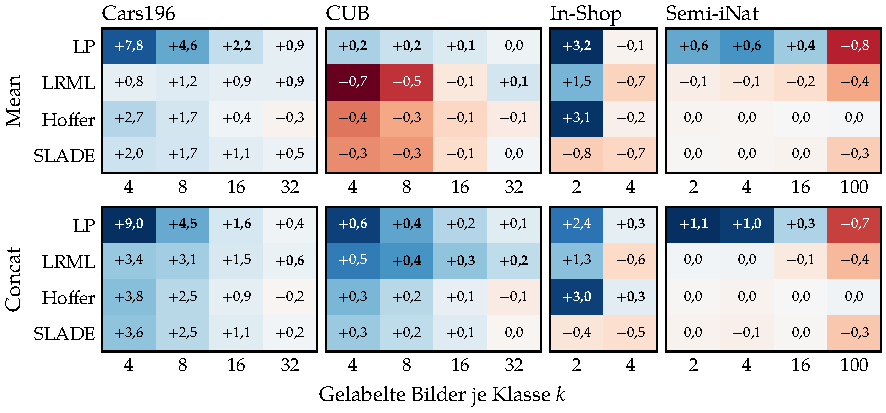
\includegraphics{neu/phase1_gewinne}
  \caption[Gewinn der \acs{SSL}-Verfahren gegenüber der supervised Referenz]{Gepaarter Gewinn der Test-\acs{MAP@R} der vier \acs{SSL}-Verfahren gegenüber der \UEBL in Prozentpunkten, gemittelt über die fünf Seeds und die fünf Verlustfunktionen. Fett: größter gerundeter Gewinn je Datensatz und Budget, getrennt nach Mean und Concat, sofern er positiv ist. Farbskala je Datensatz symmetrisch um null.}
  \label{fig:e:gewinne}
\end{figure}

\subsection{Cars196}

Auf Cars196 gewinnen bei kleinen Budgets alle vier Mechanismen gegenüber der \UEBL, \ac{LP} am meisten (Abbildung~\ref{fig:e:gewinne}). Bei $k=4$ gewinnt \ac{LP} als Einzelmodell im Mittel \num{7.8} Prozentpunkte, wie bei $k=8$ und $k=16$ ohne einen einzigen negativen Vergleich. Mit vier gelabelten Bildern je Klasse erreicht es das Niveau der Referenz mit 16, mit acht das der Referenz mit 32. Hoffer und \ac{SLADE} gewinnen bei $k=4$ deutlich weniger. \ac{LRML} verbessert das Einzelmodell nur wenig, das Ensemble aber um \num{3.4} Prozentpunkte. Dieser Unterschied zwischen dem Einzelmodell und dem Ensemble wird in Abschnitt~\ref{sec:e:faktoren} genauer betrachtet.%


\subsection{\acs{CUB}}

Auf \ac{CUB} bleiben alle mittleren Unterschiede unter einem Prozentpunkt (Abbildung~\ref{fig:e:gewinne}). Als Einzelmodelle liegen \ac{LRML}, Hoffer und \ac{SLADE} bis $k=16$ im Mittel sogar unter der \UEBL, im Ensemble gewinnen alle vier Verfahren wenige Zehntel eines Prozentpunkts. Die Mechanismen verändern auf \ac{CUB} also vor allem wenig und die Einzelmodelle bleiben meist unter den unveränderten Merkmalen (Abschnitt~\ref{sec:e:ausgangslage}).%


\subsection{In-Shop}

Auf In-Shop gewinnen bei $k=2$ \ac{LP} und Hoffer am meisten, je gut drei Prozentpunkte als Einzelmodell und in allen 25 Vergleichen (Abbildung~\ref{fig:e:gewinne}, Tabelle~\ref{tab:anhang:negativ}). \ac{LRML} gewinnt etwa halb so viel, \ac{SLADE} ist im Mittel schlechter als die \UEBL. Bei $k=4$, wenn bereits \qty{60}{\percent} des Trainingspools gelabelt sind, verschwindet der Gewinn bei allen Verfahren. Obwohl die DINOv2-Merkmale auf In-Shop ohne Training viel schwächer sind als auf Cars196, fällt der größte Gewinn kleiner aus.%


\subsection{Semi-iNat-2021}

Auf Semi-iNat-2021 hilft nur \ac{LP} (Abbildung~\ref{fig:e:gewinne}). Bis $k=16$ ist \ac{LP} in jedem gepaarten Vergleich besser als die \UEBL, bei $k=2$ um \num{0.6} Prozentpunkte als Einzelmodell. Mit zwei Labels je Art erreicht \ac{LP} das Niveau der Referenz mit vier. Bei $k=100$ kehrt sich der Gewinn in einen Verlust um. \ac{LRML}, Hoffer und \ac{SLADE} bleiben bei allen Budgets im Mittel über die Verlustfunktionen innerhalb eines halben Prozentpunkts um die \UEBL.%


Trotz des geringen Unterschieds zwischen der Leistung der \UEBL und der von \ac{LP} ist der Gewinn von \ac{LP} kein Zufall der Seeds, denn die Standardabweichung über die Seeds beträgt je Konfiguration höchstens \num{0.11} Prozentpunkte. Die Werte je Verlustfunktion stehen in Tabelle~\ref{tab:anhang:semiinat}. 

Zusammengefasst helfen ungelabelte Bilder vor allem auf Cars196 und auf In-Shop bei wenigen Labels, kaum auf \ac{CUB} und Semi-iNat-2021, wo auch zusätzliche echte Labels vergleichsweise wenig bringen (Abschnitt~\ref{sec:e:ausgangslage}). \ac{LP} gewinnt beim kleinsten Budget auf Cars196, In-Shop und Semi-iNat-2021 in jedem gepaarten Vergleich.%




\section{Einflussfaktoren}
\label{sec:e:faktoren}

\subsection{Label-Budget, Verfahren und Verlustfunktion}
\label{sec:e:beste}

Liegt ein Verfahren beim kleinsten Budget im Mittel über der \UEBL, ist sein Gewinn beim größten Budget auf allen vier Datensätzen kleiner, als Einzelmodell wie im Ensemble (Abbildung~\ref{fig:e:gewinne}). Einzige Ausnahme ist \ac{LRML} als Einzelmodell auf Cars196, dessen Gewinn bei allen Budgets zwischen \num{0.8} und \num{1.2} Prozentpunkten liegt. Am stärksten sinkt der Gewinn von \ac{LP} auf Cars196. Von $k=4$ bis $k=32$ fällt er als Einzelmodell von \num{7.8} auf \num{0.9} Prozentpunkte und im Ensemble um \qty{96}{\percent}, während der ungelabelte Pool um \qty{36}{\percent} schrumpft und die \UEBL im Ensemble um rund zehn Prozentpunkte zulegt.%

\begin{table}[tbp]
\centering\small\setlength{\tabcolsep}{4pt}
\caption[Beste Kombination aus Verfahren und Verlustfunktion]{Höchste Test-MAP@R in \% je Datensatz, Budget und Modelltyp, Mittel über die fünf Seeds. \acs{SSL}: beste der 20 Kombinationen aus den vier \acs{SSL}-Mechanismen und den fünf Verlustfunktionen (Spalten Verfahren und Verlust), \UEBL: mit der besten der fünf Verlustfunktionen.}
\label{tab:e:beste}
\begin{tabular}{@{}l *{2}{l l S[table-format=2.1] S[table-format=2.1]}@{}}
\toprule
 & \multicolumn{4}{c}{Einzelmodell (Mean)} & \multicolumn{4}{c}{Ensemble (Concat)} \\
\cmidrule(lr){2-5}\cmidrule(l){6-9}
Budget & Verfahren & Verlust & {\acs{SSL}} & {\UEBL} & Verfahren & Verlust & {\acs{SSL}} & {\UEBL} \\
\midrule
\multicolumn{9}{@{}l}{\textbf{Cars196}} \\
\quad $k=4$ & \acs{LP} & \acs{MS} & 41.5 & 34.3 & \acs{LP} & \acs{MS} & 45.6 & 36.5 \\
\quad $k=8$ & \acs{LP} & \acs{MS} & 42.6 & 38.6 & \acs{LP} & \acs{MS} & 46.1 & 41.6 \\
\quad $k=16$ & \acs{LP} & \acs{MS} & 43.3 & 41.3 & \acs{LP} & \acs{MS} & 46.3 & 44.5 \\
\quad $k=32$ & \acs{LP} & \acs{MS} & 43.4 & 43.0 & \acs{LP} & \acs{MS} & 46.4 & 45.9 \\
\midrule
\multicolumn{9}{@{}l}{\textbf{\acs{CUB}}} \\
\quad $k=4$ & \acs{LP} & \acs{MS} & 52.4 & 51.8 & \acs{LP} & \acs{MS} & 53.3 & 52.5 \\
\quad $k=8$ & \acs{LP} & \acs{MS} & 52.7 & 52.1 & \acs{LP} & \acs{MS} & 53.4 & 52.9 \\
\quad $k=16$ & \acs{LP} & \acs{MS} & 52.8 & 52.4 & \acs{LP} & \acs{MS} & 53.5 & 53.2 \\
\quad $k=32$ & \acs{LP} & \acs{MS} & 52.9 & 52.7 & \acs{LP} & \acs{MS} & 53.7 & 53.5 \\
\midrule
\multicolumn{9}{@{}l}{\textbf{In-Shop}} \\
\quad $k=2$ & \acs{LP} & ArcFace & 58.9 & 55.9 & \acs{LP} & \acs{MS} & 61.1 & 58.8 \\
\quad $k=4$ & \acs{LP} & \acs{MS} & 60.4 & 60.6 & \acs{LP} & \acs{MS} & 62.2 & 61.6 \\
\midrule
\multicolumn{9}{@{}l}{\textbf{Semi-iNat-2021}} \\
\quad $k=2$ & \acs{LP} & \acs{MS} & 35.1 & 34.1 & \acs{LP} & \acs{MS} & 35.9 & 34.6 \\
\quad $k=4$ & \acs{LP} & \acs{MS} & 35.8 & 34.8 & \acs{LP} & \acs{MS} & 36.7 & 35.5 \\
\quad $k=16$ & \acs{LP} & NT-Xent & 36.7 & 36.2 & \acs{LP} & NT-Xent & 37.6 & 37.1 \\
\quad $k=100$ & \acs{LRML} & \acs{MS} & 37.5 & 37.3 & \acs{LRML} & \acs{MS} & 38.2 & 38.0 \\
\bottomrule
\end{tabular}
\end{table}


Tabelle~\ref{tab:e:beste} stellt je Datensatz und Budget die beste Kombination aus \ac{SSL}-Verfahren und Verlustfunktion der \UEBL mit ihrer besten Verlustfunktion gegenüber. Auf Cars196 und \ac{CUB} ist das bei jedem Budget \ac{LP} mit \ac{MS}, als Einzelmodell wie im Ensemble. Dasselbe gilt auf Semi-iNat-2021 bei $k=2$ und 4 und auf In-Shop außer für das Einzelmodell bei $k=2$, bei dem \ac{LP} mit ArcFace vorn liegt. Auf Cars196 schrumpft auch der Vorsprung der besten Kombination vor der \UEBL mit jedem größeren Budget, als Einzelmodell von gut sieben Prozentpunkten bei $k=4$ auf \num{0.4} bei $k=32$. Auf In-Shop liegt bei $k=4$ als Einzelmodell und in der In-Shop-Serie bei \qty{50}{\percent} gelabelter Klassen im Ensemble die \UEBL vorn. In dieser Serie ist bis \qty{25}{\percent} \ac{LRML} mit Circle die beste Kombination.%

Im Mittel über die fünf Verfahren ist \ac{MS} in 32 der 36 Kombinationen aus Datensatz, Budget und Modelltyp die beste Verlustfunktion und für die \UEBL allein in 29. In den vier übrigen, alle im Ensemble, liegt eine andere Verlustfunktion \num{0.03} bis \num{0.12} Prozentpunkte vor \ac{MS}. Beim Budget der Hyperparametersuche liegen die beste und die schwächste Verlustfunktion im Mittel über die Verfahren auf Cars196, \ac{CUB} und Semi-iNat-2021 höchstens \num{0.9} Prozentpunkte auseinander, auf In-Shop \num{1.7} bis \num{2.0} und in der In-Shop-Serie \num{2.2} bis \num{2.7}. Auf In-Shop und in der In-Shop-Serie ist Proxy-Anchor bei jedem Budget und jedem Modelltyp die schwächste.%

Auf Cars196 gewinnt \ac{LP} bei $k=4$ als Einzelmodell mit jeder Verlustfunktion sechs bis neun Prozentpunkte, Hoffer und \ac{SLADE} je nach Verlustfunktion zwischen null und gut vier (Abbildung~\ref{fig:e:verluste}). Bei \ac{LRML} hängt dort sogar das Vorzeichen von der Verlustfunktion ab, denn mit \ac{MS} verliert es und mit den übrigen vier gewinnt es. Bei den kleinen Budgets, auf Cars196 und Semi-iNat-2021 bis $k=16$ und auf In-Shop bei $k=2$, liegt \ac{LP} dagegen als Einzelmodell im Mittel der Seeds mit jeder Verlustfunktion über der \UEBL. Für \ac{LRML}, Hoffer und \ac{SLADE} gilt das nicht. Auf In-Shop geht bei Hoffer der Unterschied zwischen den Verlustfunktionen vor allem auf die \UEBL zurück. Hoffer erreicht dort bei $k=2$ als Einzelmodell mit allen fünf zwischen \qty{57.5}{\percent} und \qty{58.1}{\percent}, die \UEBL mit Proxy-Anchor aber nur \qty{53.7}{\percent}, weniger als mit jeder anderen Verlustfunktion. Deshalb gewinnt Hoffer auf In-Shop gerade mit Proxy-Anchor am meisten, auf Cars196 dagegen am wenigsten.%


\subsection{Einzelmodell und Ensemble}

Das Ensemble ist in allen Wiederholungen mindestens so gut wie das Mittel seiner Einzelmodelle, in \ac{MAP@R} wie in \ac{RP} und auf \ac{CUB} in 491 von 500 Wiederholungen auch in \ac{P@1}. Wie viel das Ensemble gegenüber seinen Einzelmodellen gewinnt, hängt vom Verfahren ab. Auf Cars196 und \ac{CUB} ist dieser Abstand bei kleinen Budgets unter \ac{LRML} am größten. Auf Cars196 beträgt der Abstand zwischen Concat und Mean bei $k=4$ für \ac{LRML} \num{4.9} Prozentpunkte, aber für die \UEBL nur \num{2.3}. Deshalb unterscheiden sich die Aussagen für Einzelmodell und Ensemble. Mit \ac{MS} liegt \ac{LRML} bei $k=4$ als Einzelmodell in allen fünf Seeds unter der \UEBL, während es als Ensemble in allen fünf darüber liegt. Die Fold-Modelle von \ac{LRML} sind einzeln also kaum besser als die der Referenz, ergänzen sich aber stärker (Abschnitt~\ref{sec:e:phase2:concat}). \ac{LP}, Hoffer und \ac{SLADE} verbessern dagegen schon die Einzelmodelle deutlich.%


\subsection{Validierung, Test und Retrieval-Beispiele}

Die Validierung ordnet die Kombinationen weitgehend wie der Test. Auf Cars196 überschätzt sie die Gewinne aber. Dort ist die Differenz zur \UEBL in der Validierung in \CarsStat{vt-larger} von \CarsStat{vt-cells} Fällen größer als im Test, im Mittel \CarsStat{vt-dv} gegenüber \CarsStat{vt-dt}~Prozentpunkten, am stärksten bei \ac{LP} mit rund zwei Prozentpunkten. Auf \ac{CUB} ist die Differenz in 62 von 80 Fällen größer, im Mittel aber nur um \num{0.2} Prozentpunkte. Auf In-Shop, in der In-Shop-Serie und auf Semi-iNat-2021 liegen Validierung und Test im Mittel weniger als \num{0.1} Prozentpunkte auseinander. Auf Cars196 sind Gewinne in der Validierung daher nicht als gleich große Gewinne im Test zu lesen.%


\begin{figure}[tbp]
  \centering
  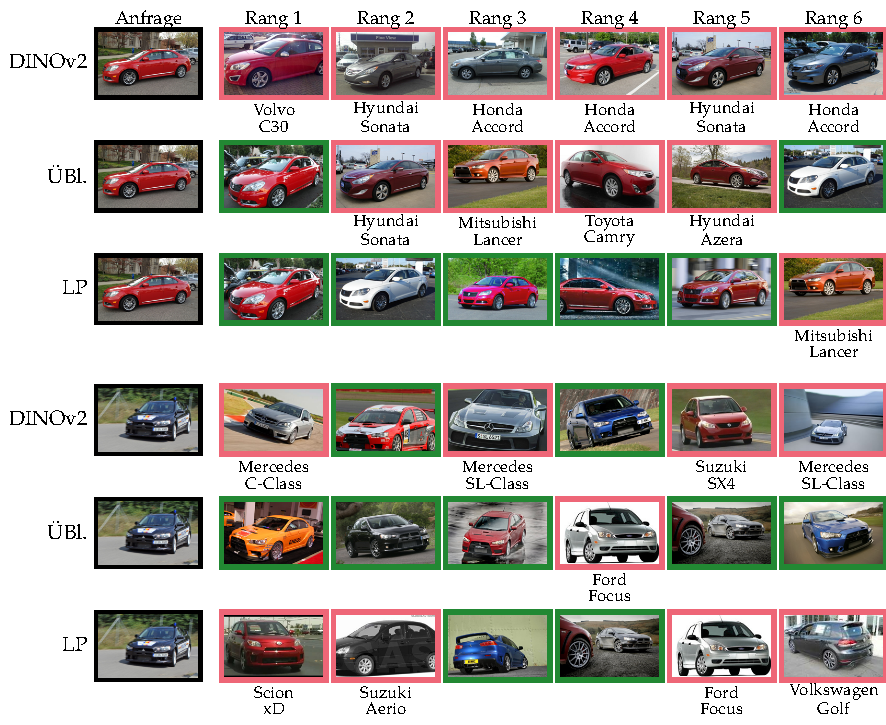
\includegraphics{neu/retrieval_ergebnisse}
  \caption[Retrieval-Beispiele auf Cars196]{Nächste Nachbarn zweier Cars196-Querys für die unveränderten DINOv2-Merkmale, die \UEBL und \acs{LP} (Circle, $k=16$, Seed~2, Concat). Grün umrandet: gleiche Klasse wie die Query, rot: andere Klasse, darunter das Modell. Oben ist \acs{LP} besser als die \UEBL (Suzuki Kizashi), unten schlechter (Mitsubishi Lancer).}
  \label{fig:e:retrieval}
\end{figure}

Abbildung~\ref{fig:e:retrieval} zeigt, wie sich die Unterschiede zwischen der \UEBL und \ac{LP} im Einzelfall äußern. Bei 32 der \num{8131} Querys findet die \UEBL höchstens zwei und \ac{LP} mindestens fünf der sechs nächsten Nachbarn richtig. Nur vier Querys zeigen das umgekehrte Muster. Aus beiden Gruppen ist je eine Limousine derselben Größenklasse gezeigt. Beim Suzuki Kizashi finden die DINOv2-Merkmale Mittelklasselimousinen anderer Hersteller ähnlicher Farbe. Die \UEBL findet neben einem richtigen Treffer ebenfalls vor allem andere Modelle und \ac{LP} findet fast nur Kizashis. Beim Mitsubishi Lancer ist es umgekehrt und \ac{LP} liefert kompakte Autos anderer Hersteller. Im Mittel über alle Querys sind \qty{64.0}{\percent} der sechs nächsten Nachbarn der DINOv2-Merkmale richtig, \qty{83.8}{\percent} bei der \UEBL und \qty{85.0}{\percent} bei \ac{LP}.

\section{Herkunft der ungelabelten Bilder}
\label{sec:e:herkunft}

In den folgenden Abschnitten stammen die ungelabelten Bilder zuerst aus Klassen ohne Labels, danach aus einem externen Datensatz.

\subsection{Bilder aus Klassen ohne Labels}
\label{sec:e:klassen}

In der zweiten In-Shop-Serie ist ein Anteil der Trainingsklassen vollständig gelabelt. Das Muster unterscheidet sich für diese Aufteilung deutlich von der $k$-Serie.

\begin{figure}[tbp]
  \centering
  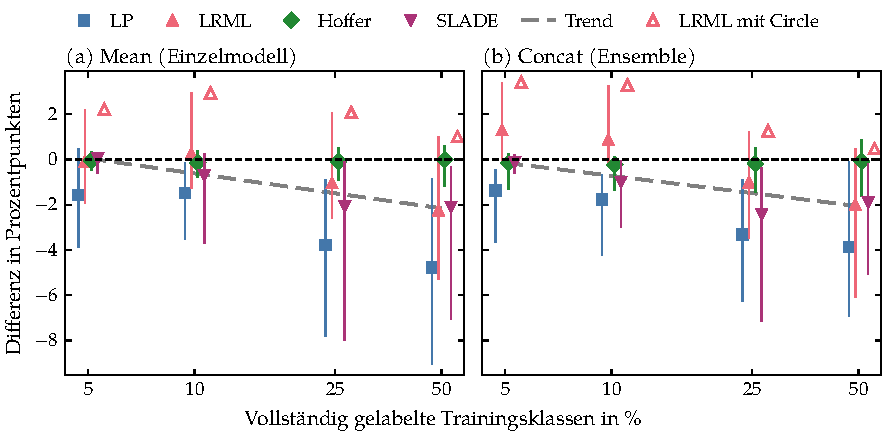
\includegraphics{neu/inshop10_gewinn}
  \caption[In-Shop mit vollständig gelabelten Klassen]{Gepaarter Gewinn der Test-\acs{MAP@R} gegenüber der \UEBL über den Anteil gelabelter Klassen auf In-Shop, (a)~Mean, (b)~Concat, Mittel über die fünf Verlustfunktionen (Striche: Spanne). Hohle Dreiecke: \acs{LRML} mit Circle. Grau gestrichelt: Trend über die vier Verfahren (lineare Anpassung an ihren Median je Anteil).}
  \label{fig:e:klassen}
\end{figure}

Stammen die ungelabelten Bilder aus Klassen ohne Labels, dann hilft nur \ac{LRML} (Abbildung~\ref{fig:e:klassen}). \ac{LP} ist bei jedem Klassenanteil schlechter als die \UEBL, Hoffer liegt nahe null und \ac{SLADE} liegt ab \qty{10}{\percent} gelabelter Klassen unter der \UEBL. \ac{LRML} gewinnt im Ensemble bei 5 und \qty{10}{\percent} gelabelten Klassen mit vier bzw.\ drei der fünf Verlustfunktionen. Als Einzelmodell liegt es dort im Mittel auf dem Niveau der \UEBL. Mit Circle gewinnt \ac{LRML} bei allen Anteilen und in allen Seeds als Einzelmodell wie im Ensemble und erreicht bei 5, 10 und \qty{25}{\percent} die höchste Ensemble-\ac{MAP@R} der Serie. Ab \qty{25}{\percent} gelabelter Klassen ist \ac{LRML} im Mittel über die Verlustfunktionen aber ebenfalls schlechter als die \UEBL. Die Mechanismen, die jedes ungelabelte Bild einer gelabelten Klasse zuordnen, profitieren hier also nicht, \ac{LRML}, das keine solche Zuordnung vornimmt, bei wenigen gelabelten Klassen dagegen schon.%

\begin{table}[tbp]
\centering
\caption[Zerlegung des Gewinns von \acs{LRML} bei Klassen ohne Labels]{Zerlegung des Gewinns von \acs{LRML} in der In-Shop-Serie mit \qty{10}{\percent} vollständig gelabelten Klassen (Seed 2): Änderung der Test-MAP@R gegenüber der regulären Konfiguration in Prozentpunkten, \UEBL und regulär absolut in \%. Varianten wie in Abschnitt \ref{sec:m:phase2}. Rauschschwelle $2\sqrt{2}\,\sigma$ aus den fünf Seeds der Phase 1 bei \qty{10}{\percent} (Abschnitt \ref{sec:m:phase2}).}
\label{tab:e:klassen:2x2}
\footnotesize\setlength{\tabcolsep}{4pt}\renewcommand{\arraystretch}{0.95}
\begin{tabular}{@{}l *{5}{S[table-format=+2.1, retain-explicit-plus]}@{}}
\toprule
{Variante} & {ArcFace} & {Circle} & {\acs{MS}} & {NT-Xent} & {Proxy-Anchor} \\
\midrule
\multicolumn{6}{@{}l}{\textit{Einzelmodell (Mean)}} \\
\quad \UEBL (MAP@R) & 48.2 & 47.7 & 48.4 & 48.1 & 48.0 \\
\quad regulär (MAP@R) & 48.4 & 50.7 & 49.2 & 46.9 & 47.4 \\
\quad Rauschschwelle & 0.9 & 0.2 & 0.5 & 0.4 & 0.5 \\
\quad Hyperparameter der \UEBL & -1.0 & -4.1 & -0.1 & +0.8 & -19.1 \\
\quad ohne ungelabelte Bilder & -0.8 & -2.5 & -1.8 & +0.5 & -0.2 \\
\addlinespace
\multicolumn{6}{@{}l}{\textit{Ensemble (Concat)}} \\
\quad \UEBL (MAP@R) & 52.5 & 52.3 & 52.9 & 51.9 & 51.9 \\
\quad regulär (MAP@R) & 52.9 & 55.4 & 54.7 & 51.8 & 51.6 \\
\quad Rauschschwelle & 1.0 & 0.4 & 1.1 & 0.6 & 0.4 \\
\quad Hyperparameter der \UEBL & +0.3 & -5.0 & -1.7 & +0.0 & -20.2 \\
\quad ohne ungelabelte Bilder & -1.0 & -2.2 & -2.2 & +0.6 & -0.1 \\
\bottomrule
\end{tabular}
\end{table}


Dass \ac{LRML} dabei die Bilder neuer Klassen selbst verwertet, zeigt die $2\times2$-Zerlegung bei \qty{10}{\percent} gelabelter Klassen (Tabelle~\ref{tab:e:klassen:2x2}). Ohne die ungelabelten Bilder verliert \ac{LRML} im Ensemble und als Einzelmodell mit Circle und \ac{MS} deutlich mehr als die Rauschschwelle, also gerade mit den beiden Verlustfunktionen, mit denen es bei diesem Anteil im Ensemble am deutlichsten gewinnt. Mit ArcFace liegt der Verlust an der Rauschschwelle. Mit \ac{NT-Xent} schneidet \ac{LRML} ohne die ungelabelten Bilder dagegen um knapp mehr als die Rauschschwelle besser ab. Mit den Hyperparametern der \UEBL verliert \ac{LRML} vor allem mit Proxy-Anchor (rund 20 Prozentpunkte) und Circle (vier bis fünf Prozentpunkte).%


Bei ähnlichem gelabeltem Anteil des Trainingspools und fast gleicher Leistung der \UEBL (\qty{54.2}{\percent} bei \qty{25}{\percent} gelabelter Klassen, \qty{54.6}{\percent} bei $k=2$) verliert \ac{LP} in dieser Serie \num{3.8} Prozentpunkte und gewinnt in der $k$-Serie \num{3.2}. Am meisten verliert \ac{LP} hier bei jedem Anteil mit ArcFace und Proxy-Anchor (Tabelle~\ref{tab:anhang:inshop10}). Mit ArcFace und Proxy-Anchor bleibt die beste Validierungs-\ac{MAP@R} nach dem Warm-up in 79 bzw.\ 80 von 80 Folds unter der besten des Warm-ups. Mit Circle sind es 66 von 80 Folds, mit \ac{MS} und \ac{NT-Xent} 0 bzw.\ 6. In der $k$-Serie tritt das mit keiner der fünf Verlustfunktionen auf. Mit \ac{MS} und \ac{NT-Xent} liegt die gewählte Konfidenzschwelle so niedrig, dass \ac{LP} von der ersten Aktualisierung an alle ungelabelten Bilder übernimmt, deren Pseudo-Labels ausnahmslos falsch sind, weil keines zu einer gelabelten Klasse gehört.%




\subsection{Externe ungelabelte Bilder}
\label{sec:e:extern}

\begin{table}[tbp]
\centering
\caption[Externe ungelabelte Bilder]{Externe ungelabelte Bilder bei vollständig gelabelten Trainingsklassen (Seed 2): gepaarter Gewinn der Test-MAP@R gegenüber der \UEBL ohne externe Bilder in Prozentpunkten, Mittel über die fünf Verlustfunktionen. Anteil: genutzter Anteil von CompCars (Cars196) bzw.\ Fashion200k (In-Shop), darunter die Bildzahl. Ohne: Kontrolle ohne externe Bilder, bei Hoffer und SLADE mit abgeschaltetem \acs{SSL}-Term. \UEBL: Test-MAP@R in \%. Fett: größter Gewinn je Spalte, sofern er positiv ist. M: Mean, C: Concat.}
\label{tab:e:extern}
\setlength{\tabcolsep}{2.9pt}
\small
\begin{tabular}{@{}ll *{10}{S[table-format=+2.1, retain-explicit-plus]}@{}}
\toprule
 & & \multicolumn{5}{c}{Cars196 + CompCars} & \multicolumn{5}{c}{In-Shop + Fashion200k} \\
\cmidrule(lr){3-7}\cmidrule(lr){8-12}
\multicolumn{2}{@{}l}{Anteil} & {ohne} & {\qty{10}{\percent}} & {\qty{25}{\percent}} & {\qty{50}{\percent}} & {\qty{100}{\percent}} & {ohne} & {\qty{5}{\percent}} & {\qty{10}{\percent}} & {\qty{25}{\percent}} & {\qty{50}{\percent}} \\
\multicolumn{2}{@{}l}{Bilder} & {\num{0}} & {\num{1654}} & {\num{4134}} & {\num{8268}} & {\num{16537}} & {\num{0}} & {\num{16917}} & {\num{33834}} & {\num{84585}} & {\num{169170}} \\
\midrule
\UEBL & M & \multicolumn{5}{c}{\num{43.1}} & \multicolumn{5}{c}{\num{60.1}} \\
 & C & \multicolumn{5}{c}{\num{45.3}} & \multicolumn{5}{c}{\num{60.9}} \\
\addlinespace
\multicolumn{2}{@{}l}{\emph{Gewinn (M)}} & & & & & & & & & & \\
LP & & +0.1 & -5.5 & -5.3 & -5.3 & -4.9 & -1.1 & -8.6 & -8.5 & -8.1 & -8.0 \\
\acs{LRML} & & \bfseries +0.7 & -0.7 & -1.4 & -2.0 & -2.3 & -1.3 & -3.8 & -4.9 & -6.4 & -8.2 \\
Hoffer & & -0.3 & -4.6 & -4.5 & -4.7 & -4.4 & -3.2 & -8.0 & -7.8 & -7.5 & -7.6 \\
SLADE & & +0.4 & -3.7 & -3.6 & -3.7 & -3.7 & -5.0 & -4.0 & -4.1 & -3.9 & -4.0 \\
\addlinespace
\multicolumn{2}{@{}l}{\emph{Gewinn (C)}} & & & & & & & & & & \\
LP & & +0.1 & -6.6 & -6.3 & -6.2 & -6.0 & -1.0 & -8.2 & -8.2 & -7.9 & -7.9 \\
\acs{LRML} & & \bfseries +0.5 & -0.6 & -1.4 & -2.2 & -3.2 & -1.1 & -3.1 & -4.0 & -6.3 & -8.1 \\
Hoffer & & -0.5 & -4.2 & -4.3 & -4.4 & -4.4 & -2.9 & -7.7 & -7.4 & -7.0 & -7.3 \\
SLADE & & +0.4 & -3.9 & -3.9 & -4.1 & -4.1 & -4.7 & -3.8 & -3.9 & -3.7 & -3.7 \\
\bottomrule
\end{tabular}
\end{table}


Mit allen Labels der Trainingsklassen und einem externen ungelabelten Pool wie in der Originalarbeit von \ac{SLADE} liegt kein Mechanismus im Mittel über die Verlustfunktionen über der \UEBL (Tabelle~\ref{tab:e:extern}, Einzelwerte in den Tabellen~\ref{tab:anhang:extern:cars} und~\ref{tab:anhang:extern:inshop}). Auf In-Shop liegen 79 der 80 gepaarten Vergleiche um mehr als die Rauschschwelle unter der \UEBL, auf Cars196 71. \ac{LP}, Hoffer und \ac{SLADE} verlieren fast unabhängig von der Größe des Pools mehrere Prozentpunkte und \ac{LRML} verliert mit wachsendem Pool mehr. Über der \UEBL liegt mit externem Pool nur \ac{LRML} mit \ac{NT-Xent} auf Cars196 bei 10 und \qty{25}{\percent}, allerdings unter der Rauschschwelle.%


Ohne externe Bilder liegen \ac{LP}, Hoffer und \ac{SLADE} auf Cars196 auf dem Niveau der \UEBL, \ac{LRML} liegt leicht darüber (Spalte \enquote{ohne} in Tabelle~\ref{tab:e:extern}). Die Verluste auf Cars196 entstehen also erst mit den externen Bildern, bei \ac{LP}, Hoffer und \ac{SLADE} zugleich mit ihrem Mechanismus, der in der Kontrolle fehlt. Auf In-Shop liegen dagegen schon diese Kontrollen im Mittel unter der \UEBL, mit \ac{LP} und \ac{LRML} um gut einen Prozentpunkt, mit Hoffer und \ac{SLADE} um mehrere Prozentpunkte. Bei \ac{LP} geht dieses Mittel allein auf ArcFace zurück (\num{-9.7} Prozentpunkte). Mit den übrigen vier Verlustfunktionen liegt die Kontrolle um mehr als die Rauschschwelle über der \UEBL. Bei \ac{SLADE} bestimmen es Proxy-Anchor (\num{-18.3}) und ArcFace (\num{-8.1}). Andere Nachbar- und Clusterzahlen ändern das Bild auf Cars196 kaum (Tabelle~\ref{tab:anhang:extern:sweeps}). In den verwendeten Konfigurationen von \ac{LP} stammen auf Cars196 \num{12.5} bis \qty{25}{\percent} jedes Batches aus den gelabelten Bildern, auf In-Shop \qty{50}{\percent}.%



\section{Worauf der Nutzen beruht}
\label{sec:e:phase2}
Die Ablationen der Phase~2 laufen auf Cars196 bei $k=16$ und $k=8$ und auf In-Shop bei $k=2$, jeweils mit allen vier Mechanismen und allen fünf Verlustfunktionen. Wo nicht anders angegeben, beziehen sich die folgenden Abschnitte auf Cars196 mit $k=16$ und auf In-Shop.  Tabelle~\ref{tab:e:ablationen:verluste} gibt für jede Kombination die Änderung gegenüber der regulären Konfiguration an, Anhang~\ref{chap:anhang:phase2} enthält alle Einzelwerte. Als Befund gilt ein Unterschied erst oberhalb der Rauschschwelle aus Abschnitt~\ref{sec:m:phase2}, die für jede Kombination aus Mechanismus und Verlustfunktion getrennt bestimmt wird.

\begin{table}[tbp]
\centering
\caption[Ablationen der Phase 2 auf Cars196 und In-Shop]{Ablationen der Phase 2 auf Cars196 und In-Shop (Seed 2): Änderung der Test-MAP@R (Mean) gegenüber der regulären Konfiguration in Prozentpunkten, \UEBL und regulär absolut in \%. Eingriffe wie in Tabelle \ref{tab:phase2:eingriffe} und Abschnitt \ref{sec:m:phase2}, eingefroren: Pseudo-Labels bzw.\ Graph. Fett: Änderung größer als die Rauschschwelle. Ohne Warm-up: gleich der regulären Konfiguration, wo Phase 1 kein Warm-up gewählt hat. Arc: ArcFace, Cir: Circle, NT: NT-Xent, PA: Proxy-Anchor.}
\label{tab:e:ablationen:verluste}
\footnotesize\setlength{\tabcolsep}{3.2pt}\setlength{\hfuzz}{1.2pt}\renewcommand{\arraystretch}{0.95}
\begin{tabular}{@{}l *{5}{S[table-format=+2.1, retain-explicit-plus]} @{\hspace{12pt}} *{5}{S[table-format=+2.1, retain-explicit-plus]}@{}}
\toprule
& \multicolumn{5}{c}{\textbf{Cars196} ($k=16$)} & \multicolumn{5}{c}{\textbf{In-Shop} ($k=2$)} \\
\cmidrule(lr){2-6}\cmidrule(l){7-11}
{Variante} & {Arc} & {Cir} & {\acs{MS}} & {NT} & {PA} & {Arc} & {Cir} & {\acs{MS}} & {NT} & {PA} \\
\midrule
\textit{\UEBL (MAP@R)} & 40.3 & 39.1 & 40.8 & 39.2 & 39.2 & 54.8 & 54.7 & 56.1 & 54.6 & 53.8 \\
\midrule
\multicolumn{11}{@{}l}{\textbf{LP}} \\
\quad\textit{regulär (MAP@R)} & 41.9 & 42.3 & 43.3 & 41.4 & 42.6 & 58.9 & 57.8 & 58.8 & 58.0 & 56.3 \\
\quad\textit{Rauschschwelle} & 0.8 & 0.5 & 0.6 & 0.6 & 0.3 & 0.1 & 0.3 & 0.2 & 0.4 & 0.4 \\
\cmidrule{1-11}
\quad SSL-Mechanismus abgeschaltet & \bfseries -4.5 & \bfseries -3.2 & \bfseries -2.7 & \bfseries -2.2 & \bfseries -2.7 & \bfseries -10.8 & \bfseries -3.1 & \bfseries -3.0 & \bfseries -4.2 & \bfseries -3.4 \\
\quad Hyperparameter der \UEBL & -0.5 & -0.5 & +0.5 & +0.1 & \bfseries -2.4 & \bfseries -0.7 & \bfseries -1.0 & +0.2 & \bfseries -0.7 & \bfseries -2.6 \\
\quad ohne Warm-up & \bfseries -1.0 & +0.1 & -0.4 & +0.0 & +0.0 & -0.1 & -0.1 & \bfseries +0.2 & -0.1 & \bfseries -0.4 \\
\addlinespace[2pt]
\quad eingefroren & -0.3 & \bfseries -0.9 & \bfseries -0.7 & -0.2 & \bfseries -1.4 & \bfseries -11.5 & \bfseries -2.5 & \bfseries -0.7 & \bfseries -2.2 & \bfseries -1.3 \\
\quad Graph umverdrahtet & \bfseries -14.2 & \bfseries -8.6 & \bfseries -12.3 & \bfseries -6.3 & \bfseries -10.0 & \bfseries -13.4 & \bfseries -10.2 & \bfseries -9.5 & \bfseries -11.5 & \bfseries -8.9 \\
\quad Oracle-Kanten entfernt & -0.2 & \bfseries +0.9 & +0.6 & \bfseries +1.2 & \bfseries +1.0 & \bfseries -8.2 & \bfseries +2.2 & \bfseries +1.4 & \bfseries +1.7 & \bfseries +2.0 \\
\quad zufällige Kanten entfernt & -0.1 & +0.2 & -0.4 & +0.2 & +0.1 & \bfseries -22.6 & \bfseries -4.1 & +0.2 & +0.1 & -0.1 \\
\midrule
\multicolumn{11}{@{}l}{\textbf{\acs{LRML}}} \\
\quad\textit{regulär (MAP@R)} & 40.9 & 40.9 & 40.4 & 39.9 & 41.7 & 58.0 & 57.6 & 56.6 & 55.7 & 53.7 \\
\quad\textit{Rauschschwelle} & 0.5 & 0.7 & 1.1 & 0.7 & 0.5 & 1.3 & 0.3 & 0.7 & 0.4 & 0.7 \\
\cmidrule{1-11}
\quad SSL-Mechanismus abgeschaltet & \bfseries -5.3 & \bfseries -2.1 & \bfseries -4.4 & \bfseries -3.1 & \bfseries -3.1 & \bfseries -11.0 & \bfseries -4.6 & \bfseries -2.5 & \bfseries -2.6 & \bfseries -2.7 \\
\quad ohne ungelabelte Bilder & \bfseries -3.1 & -0.4 & \bfseries -1.9 & -0.7 & \bfseries -1.1 & \bfseries -3.3 & \bfseries -4.1 & \bfseries -2.8 & \bfseries -2.5 & \bfseries -2.3 \\
\quad Hyperparameter der \UEBL & \bfseries -4.1 & +0.0 & +0.1 & \bfseries -3.2 & \bfseries -3.8 & \bfseries -5.6 & \bfseries -1.6 & +0.6 & \bfseries -1.0 & +0.4 \\
\quad ohne Warm-up & \bfseries -9.6 & -0.7 & \bfseries -2.2 & \bfseries -6.4 & \bfseries -2.1 & \bfseries -8.4 & -0.3 & -0.3 & -0.1 & \bfseries +0.7 \\
\addlinespace[2pt]
\quad eingefroren & -0.5 & -0.2 & -0.6 & +0.1 & -0.1 & \bfseries -1.3 & \bfseries -1.8 & -0.2 & -0.3 & \bfseries -2.3 \\
\quad Graph umverdrahtet & \bfseries -5.1 & \bfseries -2.2 & \bfseries -5.6 & \bfseries -2.8 & \bfseries -3.2 & \bfseries -11.4 & \bfseries -11.6 & \bfseries -4.4 & \bfseries -4.9 & \bfseries -2.6 \\
\quad Oracle-Kanten entfernt & +0.4 & +0.5 & +0.8 & +0.6 & \bfseries +0.7 & +1.2 & \bfseries +1.4 & \bfseries +0.9 & \bfseries +1.2 & \bfseries +0.7 \\
\quad zufällige Kanten entfernt & +0.2 & +0.1 & -0.3 & +0.3 & +0.0 & -0.1 & -0.1 & +0.1 & +0.1 & +0.1 \\
\midrule
\multicolumn{11}{@{}l}{\textbf{Hoffer}} \\
\quad\textit{regulär (MAP@R)} & 40.5 & 40.6 & 39.5 & 40.3 & 40.6 & 57.7 & 58.1 & 57.9 & 58.2 & 57.6 \\
\quad\textit{Rauschschwelle} & 0.3 & 0.4 & 0.5 & 0.7 & 0.5 & 0.2 & 0.2 & 0.2 & 0.2 & 0.3 \\
\cmidrule{1-11}
\quad SSL-Mechanismus abgeschaltet & \bfseries -1.3 & \bfseries -1.7 & \bfseries -0.9 & \bfseries -2.2 & \bfseries -1.1 & \bfseries -5.0 & \bfseries -3.7 & \bfseries -4.8 & \bfseries -6.2 & \bfseries -5.7 \\
\quad ohne ungelabelte Bilder & \bfseries -2.3 & \bfseries -1.3 & \bfseries -1.0 & \bfseries -1.8 & \bfseries -1.3 & \bfseries -4.1 & \bfseries -3.6 & \bfseries -4.0 & \bfseries -3.5 & \bfseries -4.0 \\
\quad Hyperparameter der \UEBL & +0.1 & \bfseries -1.3 & -0.2 & -0.7 & \bfseries -1.6 & \bfseries -0.6 & \bfseries -0.6 & \bfseries -0.9 & \bfseries -1.1 & \bfseries -1.0 \\
\quad ohne Warm-up & \bfseries -0.3 & \bfseries -1.0 & \bfseries -0.6 & -0.2 & +0.0 & \bfseries -0.5 & -0.1 & \bfseries -0.2 & -0.2 & +0.0 \\
\midrule
\multicolumn{11}{@{}l}{\textbf{SLADE}} \\
\quad\textit{regulär (MAP@R)} & 40.2 & 41.6 & 41.7 & 40.6 & 40.4 & 53.7 & 54.8 & 54.5 & 54.1 & 53.7 \\
\quad\textit{Rauschschwelle} & 1.0 & 0.6 & 1.0 & 0.3 & 0.6 & 1.4 & 0.4 & 0.4 & 0.5 & 0.9 \\
\cmidrule{1-11}
\quad SSL-Mechanismus abgeschaltet & -0.7 & \bfseries -3.1 & \bfseries -1.5 & \bfseries -2.3 & \bfseries -1.5 & -1.0 & -0.1 & \bfseries -1.8 & +0.0 & \bfseries -10.6 \\
\quad ohne ungelabelte Bilder & -0.2 & \bfseries -3.5 & -0.8 & \bfseries -1.8 & \bfseries -0.9 & +0.3 & -0.3 & \bfseries -0.5 & +0.1 & +0.0 \\
\quad Hyperparameter der \UEBL & \bfseries -4.5 & -0.5 & \bfseries -2.8 & \bfseries -5.3 & \bfseries -2.1 & \bfseries -7.1 & \bfseries -1.4 & \bfseries -3.4 & -0.3 & \bfseries -1.6 \\
\quad ohne Warm-up & \bfseries -1.2 & \bfseries -2.1 & -0.4 & \bfseries -1.4 & +0.0 & +0.0 & -0.2 & -0.1 & +0.1 & -0.1 \\
\bottomrule
\end{tabular}
\end{table}


\subsection{Hyperparameter, Term oder ungelabelte Bilder?}
\label{sec:e:2x2}

Die \ac{SSL}-Konfigurationen wurden separat optimiert. Abbildung~\ref{fig:e:2x2:verluste} zeigt die Varianten der $2\times2$-Zerlegung und die Kontrolle mit abgeschaltetem \ac{SSL}-Term als Differenz zur \UEBL.

Die reguläre Konfiguration übertrifft die \UEBL in 26 der 40 Kombinationen um mehr als die Rauschschwelle (Abbildung~\ref{fig:e:2x2:verluste}). Auf Cars196 gewinnt \ac{LP} mit allen fünf Verlustfunktionen, Hoffer und \ac{SLADE} mit je drei und \ac{LRML} mit zwei. Auf In-Shop gewinnen \ac{LP} und Hoffer mit allen fünf, \ac{LRML} mit drei und \ac{SLADE} mit keiner. Im Mittel der fünf Seeds der Phase~1 liegen sechs der 14 Kombinationen ohne Gewinn über der \UEBL (Anhang~\ref{chap:anhang:ergebnisse}).%


\begin{figure}[tbp]
  \centering
  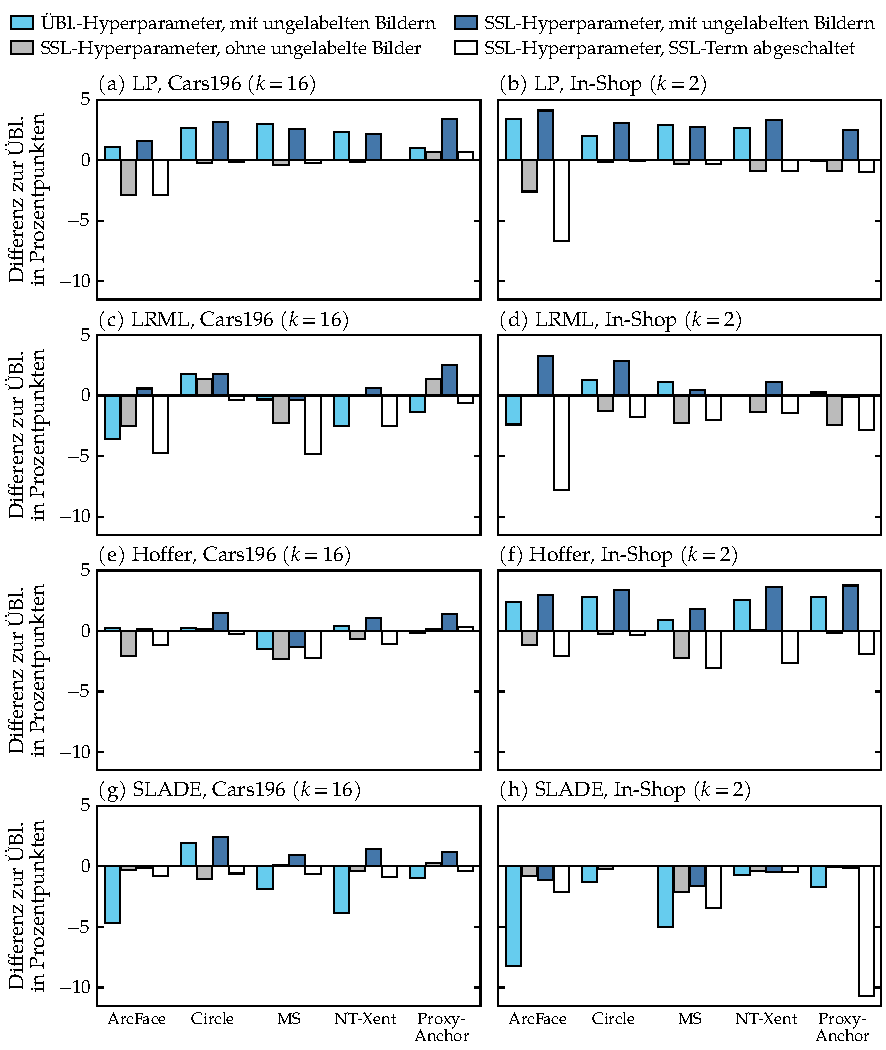
\includegraphics{neu/phase2_2x2_verluste}
  \caption[Zerlegung des Gewinns nach Hyperparametern, \acs{SSL}-Term und ungelabelten Bildern]{Zerlegung des Gewinns mit allen fünf Verlustfunktionen auf Cars196 ($k=16$, links) und In-Shop ($k=2$, rechts), zeilenweise für \acs{LP}, \acs{LRML}, Hoffer und \acs{SLADE}: Test-\acs{MAP@R} der Einzelmodelle als Differenz zur \UEBL, ein Seed. Varianten wie in Tabelle~\ref{tab:m:2x2}, dazu die Kontrolle mit abgeschaltetem \acs{SSL}-Term (Tabelle~\ref{tab:phase2:eingriffe}).}
  \label{fig:e:2x2:verluste}
\end{figure}

Die abweichenden Hyperparameter allein erklären den Gewinn nicht. Die ungelabelten Bilder leisten in den meisten Kombinationen einen eigenen Beitrag. Mit den \ac{SSL}-Hyperparametern senkt das Entfernen der ungelabelten Bilder die Leistung in 37 der 40 Kombinationen, in 32 um mehr als die Rauschschwelle. Die Kontrolle mit denselben Hyperparametern und abgeschaltetem \ac{SSL}-Term liegt dagegen nur in einer Kombination um mehr als die Rauschschwelle über der \UEBL und in 25 darunter. Ohne den Term sind die \ac{SSL}-Hyperparameter also oft sogar schlechter als die der \UEBL.%


Was der \ac{SSL}-Term ohne ungelabelte Bilder bewirkt, zeigt der Vergleich der Variante ohne ungelabelte Bilder mit der Kontrolle mit abgeschaltetem \ac{SSL}-Term (Abschnitt~\ref{sec:m:phase2}). In 18 der 40 Kombinationen liegt die Variante ohne ungelabelte Bilder um mehr als die Rauschschwelle über dieser Kontrolle. Das gilt bei \ac{LRML} auf Cars196 für alle fünf Verlustfunktionen und bei Hoffer auf In-Shop für vier, bei \ac{LP} nur in einer Kombination.

Für \ac{LRML} auf Cars196 enthält der Pool dieser Variante bei $k=16$ höchstens 15 weitere Bilder derselben Klasse je Bild. Bei den gewählten 39 bis 81 Nachbarn muss deshalb schon durch die Konstruktion die Mehrheit der Nachbarschaftsbeziehungen zu anderen Klassen führen. In sieben der 18 Kombinationen bleibt die Variante ohne ungelabelte Bilder um mehr als die Rauschschwelle unter der \UEBL.%


Die Variante mit den Hyperparametern der \UEBL misst den Term und die ungelabelten Bilder gemeinsam (Abschnitt~\ref{sec:m:phase2}). Auf Cars196 liegt sie um mehr als die Rauschschwelle über der \UEBL bei \ac{LP} mit allen fünf Verlustfunktionen, bei \ac{LRML} und \ac{SLADE} nur mit Circle und bei Hoffer mit keiner. In sechs der 15 Kombinationen von \ac{LRML}, Hoffer und \ac{SLADE} gewinnt die reguläre Konfiguration auf Cars196 also nur mit den eigens abgestimmten Hyperparametern. Auf In-Shop liegt sie dagegen bei \ac{LP} mit vier, bei Hoffer mit allen fünf, bei \ac{LRML} mit zwei und bei \ac{SLADE} mit keiner Verlustfunktion um mehr als die Rauschschwelle über der \UEBL. Da dort ohne ungelabelte Bilder keine Kombination über der \UEBL liegt, stammt der Gewinn von \ac{LP}, \ac{LRML} und Hoffer auf In-Shop von den ungelabelten Bildern. Bei \ac{SLADE} ändert das Entfernen der ungelabelten Bilder die Leistung auf In-Shop nur in einer Kombination um mehr als die Rauschschwelle.%

Bei $k=8$ (Tabelle~\ref{tab:anhang:phase2:k8} in Anhang~\ref{chap:anhang:phase2}) übertrifft die reguläre Konfiguration der \ac{SSL}-Methoden die \UEBL in 18 der 20 Kombinationen um mehr als die Rauschschwelle, das Entfernen der ungelabelten Bilder kostet in allen 20 Leistung und die Kontrolle mit abgeschaltetem \ac{SSL}-Term liegt nur bei \ac{LP} mit Proxy-Anchor über der \UEBL. Auch bei $k=8$ tragen also die ungelabelten Bilder und die \ac{SSL}-Methoden den Gewinn und nicht die separat gewählten Hyperparameter allein.%


\subsection{Qualität der Pseudo-Labels}
\label{sec:e:pseudolabels}

Die gewählte Konfidenzschwelle liegt meist so niedrig, dass \ac{LP} schon bei der ersten Aktualisierung fast jedes ungelabelte Bild übernimmt (Mittel über die vier Folds, solange alle trainieren). Auf Cars196 sind diese Pseudo-Labels anfangs zu \qty{77}{\percent} bis \qty{84}{\percent} richtig, auf In-Shop zu \qty{60}{\percent} bis \qty{69}{\percent}. Bis zum Ende des Trainings steigt ihre Genauigkeit, auf Cars196 auf \qty{85}{\percent} bis \qty{87}{\percent}. Eine Ausnahme ist Circle auf Cars196, wo die Konfidenzschwelle anfangs gut ein Drittel der Bilder ausschließt. Eine weitere Ausnahme ist ArcFace auf In-Shop, wo \ac{LP} anfangs nur \qty{5}{\percent} der Bilder übernimmt. Obwohl auf In-Shop am Ende noch rund ein Viertel der Pseudo-Labels falsch ist, liegt \ac{LP} dort mit jeder Verlustfunktion über der \UEBL.%


Auf Semi-iNat-2021 übernimmt \ac{LP} bei $k=2$ bei der ersten Aktualisierung \qty{82}{\percent} bis \qty{100}{\percent} der ungelabelten Bilder. Die Pseudo-Labels dieser Bilder sind zu \qty{57}{\percent} bis \qty{71}{\percent} richtig, ein ähnlicher Anteil wie anfangs auf In-Shop. \ac{LP} gewinnt auf Semi-iNat-2021 als Einzelmodell jedoch nur \num{0.6} Prozentpunkte, auf In-Shop dagegen \num{3.2} (Abschnitt~\ref{sec:e:phase1}). Bis zum Ende des Trainings ändert sich der Anteil richtiger Pseudo-Labels um höchstens \num{6.0} Prozentpunkte und liegt dann bei \qty{63}{\percent} bis \qty{71}{\percent}. Bei $k=100$ sind anfangs \qty{79}{\percent} bis \qty{97}{\percent} und am Ende \qty{80}{\percent} bis \qty{96}{\percent} der übernommenen Pseudo-Labels richtig. Dennoch liegt \ac{LP} dort in allen 25 Vergleichen unter der \UEBL.%


\begin{figure}[tbp]
  \centering
  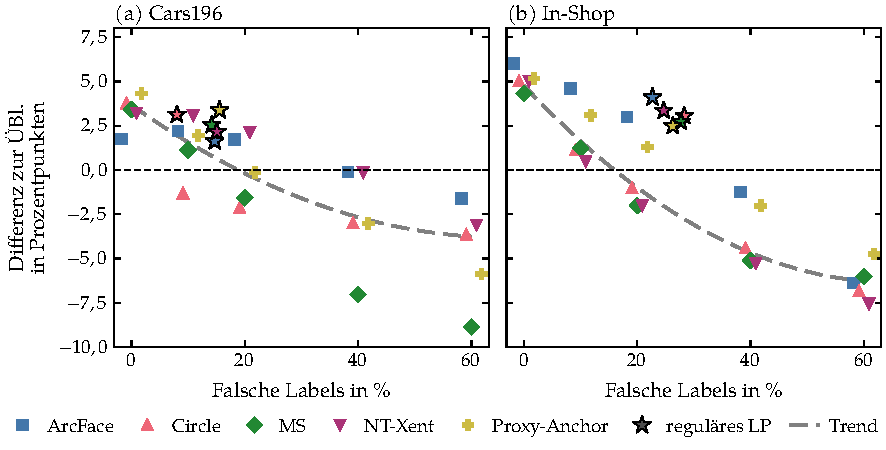
\includegraphics{neu/phase2_lp_qualitaet}
  \caption[Wirkung falscher Pseudo-Labels von \acs{LP}]{Oracle-Pseudo-Labels von \acs{LP}, von denen ein Anteil zufällig falsch ist, mit allen fünf Verlustfunktionen auf (a)~Cars196 ($k=16$) und (b)~In-Shop ($k=2$), ein Seed, als Differenz zur \UEBL. Sterne: reguläres \acs{LP} an seiner über Epochen und Folds gemittelten Fehlerrate. Grau gestrichelt: Trend über die Verlustfunktionen (quadratische Anpassung an ihren Median je Anteil).}
  \label{fig:e:lpqualitaet}
\end{figure}

Wo die falschen Pseudo-Labels liegen und was sich an ihnen während des Trainings ändert, zeigt Abbildung~\ref{fig:e:lpcars} für Cars196 an einem Fold mit Circle bei $k=16$. Abbildung~\ref{fig:e:lpcars}a zeigt die Embeddings und die Pseudo-Labels nach der ersten Epoche mit \ac{LP}. Auf Cars196 bilden nach dem Warm-up viele Klassen schon kompakte Gruppen, deren ungelabelte Bilder fast alle ein richtiges Pseudo-Label erhalten. Bis zum Ende des Trainings steigt die Abdeckung von \qty{63}{\percent} auf \qty{86}{\percent}, während die Genauigkeit der übernommenen Pseudo-Labels von \qty{94}{\percent} auf \qty{92}{\percent} sinkt. Die schon übernommenen Pseudo-Labels ändern sich dagegen kaum. Fast alle richtigen bleiben richtig und die meisten falschen behalten ihre falsche Klasse.%


\begin{figure}[tbp]
  \centering
  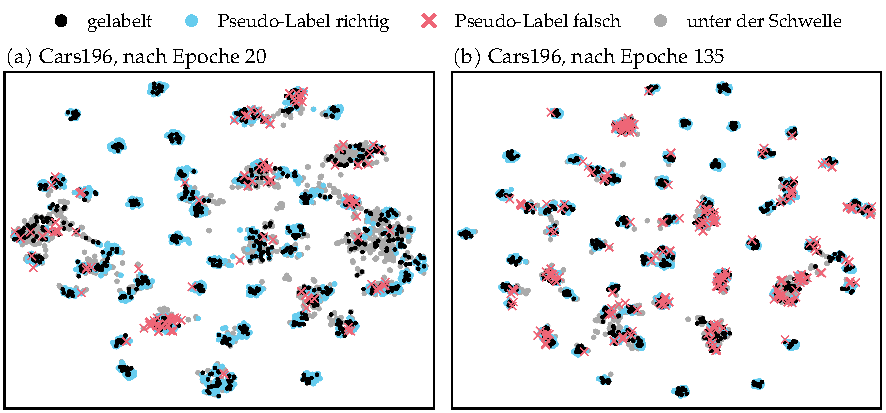
\includegraphics{neu/lp_cars}
  \caption[Label Propagation in einem Graphlauf auf Cars196]{Pseudo-Labels von \acs{LP} in einem Graphlauf auf Cars196 (Circle, $k=16$, Seed~2, Fold~0), \acs{t-SNE} der 4000 verfolgten Bilder des Trainingspools. Gezeigt sind die Pseudo-Labels, die das Training für die jeweils folgende Epoche übernimmt, berechnet aus dem Modell (a)~nach Epoche~20, der ersten nach dem Warm-up aus den Epochen 0 bis 19, (b)~nach Epoche~135 (Training bis Epoche~140). Ob ein Pseudo-Label richtig ist, zeigen die verdeckten Labels. Konfidenzschwelle \num{0.81}. Jede Teilabbildung beruht auf einer eigenen \acs{t-SNE}-Darstellung, die Lage einzelner Gruppen ist zwischen den Teilabbildungen daher nicht vergleichbar.}
  \label{fig:e:lpcars}
\end{figure}

Mit allen fünf Verlustfunktionen nennen die meisten falschen Pseudo-Labels auf Cars196 ein Modell desselben Herstellers. Über alle vier Folds ($k=16$) sind es je nach Verlustfunktion und Fold \qty{67}{\percent} bis \qty{88}{\percent} bei der ersten Aktualisierung, während bei zufälliger Verwechslung höchstens \qty{18}{\percent} zu erwarten wären.

Im entsprechenden Graphlauf auf Semi-iNat-2021 hat die Suche kein Warm-up gewählt, sodass \ac{LP} die ersten Pseudo-Labels aus dem Head vor dem Training berechnet und fast jedes ungelabelte Bild übernimmt. Anders als auf Cars196 wechselt bis zum Ende des Trainings etwa jedes siebte Pseudo-Label die Art. Nur zwei von fünf Wechseln berichtigen dabei ein falsches Pseudo-Label, sodass die Genauigkeit nur von \qty{74}{\percent} auf \qty{78}{\percent} steigt. Das Training ändert auf Cars196 also mit Circle vor allem, welche Bilder ein Pseudo-Label erhalten, mit den übrigen Verlustfunktionen dagegen, wie viele davon richtig sind. Auf Semi-iNat-2021 ändert es vor allem, welche Art die Pseudo-Labels nennen.%

Abbildung~\ref{fig:e:lpqualitaet} stellt den Fehlern von \ac{LP} auf Cars196 und In-Shop kontrollierte Fehler gegenüber. Erhalten genau die von \ac{LP} übernommenen Bilder ihr wahres Label, steigt die Leistung gegenüber der regulären Konfiguration auf Cars196 mit vier Verlustfunktionen um bis zu \num{1.1} Prozentpunkte und auf In-Shop mit allen fünf um bis zu \num{2.7}. Zufällig falsche Labels schaden auf In-Shop mit jeder Verlustfunktion deutlich. Auf Cars196 hängt der Schaden von der Verlustfunktion ab, mit Circle, \ac{MS} und Proxy-Anchor machen \qty{20}{\percent} zufällig falscher Labels den Gewinn zunichte, mit ArcFace und \ac{NT-Xent} liegt \ac{LP} auch dann noch über der \UEBL.%


Die vorab festgelegte Erwartung, dass reguläres \ac{LP} auf der Kurve der zufälligen Fehler liegt, trifft auf Cars196 nur mit ArcFace und \ac{NT-Xent} zu, wo schon zufällige Fehler kaum schaden. Mit den übrigen drei Verlustfunktionen auf Cars196 und mit allen fünf auf In-Shop liegt reguläres \ac{LP} über der Kurve, auf In-Shop um bis zu \num{6.1} Prozentpunkte. Mit der Fehlerrate der per Validierung gewählten Epoche statt der über alle Epochen gemittelten ändert sich der Abstand zur Kurve um weniger als einen halben Prozentpunkt. Reguläres \ac{LP} liegt dort also über den Läufen mit zufälligen Fehlern gleicher mittlerer Häufigkeit. Worauf dieser Abstand beruht, trennt der Vergleich nicht, denn die Varianten unterscheiden sich auch in den betroffenen Bildern und im Verlauf des Trainings.%


\subsection{Nachbarschaftsstruktur}
\label{sec:e:nachbarschaft}

Ob die konkrete Nachbarschaft der Daten den Gewinn trägt, prüfen Eingriffe in den Graphen von \ac{LP} und \ac{LRML}. Ein unter Erhalt der Knotengrade zufällig umverdrahteter Graph lässt die Leistung in allen 20 Kombinationen einbrechen, bei \ac{LP} um mindestens \num{6.3} Prozentpunkte. Beide Mechanismen liegen damit in jeder Kombination unter der \UEBL, nur \ac{LRML} mit Circle auf Cars196 innerhalb der Rauschschwelle. Ein beliebiger Zusatzterm hilft also nicht und ein Graph ohne Bezug zu den Daten schadet.%


Ein reinerer Graph hilft. Werden alle Kanten zwischen verschiedenen Klassen entfernt, steigt die Leistung in 18 der 20 Kombinationen, vor allem bei \ac{LP} und bei \ac{LRML} auf In-Shop über der Rauschschwelle. Die Ausnahme ist \ac{LP} mit ArcFace, das auf In-Shop um \num{8.2} Prozentpunkte verliert. Wird stattdessen dieselbe Zahl zufälliger Kanten entfernt, ändert sich die Leistung in 18 der 20 Kombinationen kaum. Nur \ac{LP} auf In-Shop verliert dabei mit Circle und ArcFace deutlich. Bei Circle erklärt die Zahl der entfernten Kanten das allein nicht, denn das Entfernen verschiedenklassiger Kanten hilft dort. Mit ArcFace bricht \ac{LP} auf In-Shop bei den meisten Eingriffen ein (Abschnitt~\ref{sec:e:sweeps}).%


 Auf Cars196 werden die Graphen von \ac{LP} und \ac{LRML} durch das Training um \num{29.5} bis \num{44.4} Prozentpunkte reiner. Danach verlaufen aber noch \qty{15}{\percent} bis \qty{40}{\percent} ihrer Kanten zwischen verschiedenen Klassen, genau die Kanten, die der Eingriff mit den verdeckten Labels entfernt. Auf In-Shop begrenzt die Klassengröße die Reinheit großer Graphen. In den Graphen von \ac{LP} mit ArcFace und Circle, die 83 bzw.\ 95 Nachbarn verwenden, verlaufen nach dem Training weniger als \qty{10}{\percent} der Kanten innerhalb einer Klasse. Beide Eingriffe entfernen deshalb über \qty{90}{\percent} der Kanten. Der Eingriff mit den verdeckten Labels behält dabei alle Kanten innerhalb einer Klasse, die zufällige Kontrolle entfernt auch von diesen über \qty{90}{\percent}. Das passt dazu, dass \ac{LP} mit Circle nur in der zufälligen Kontrolle einbricht. Kleine Graphen mit zwei bis sechs Nachbarn sind auf In-Shop nach dem Training zu mehr als der Hälfte rein. Auf Semi-iNat-2021 sind die Graphen schon vor dem Training zu mehr als der Hälfte rein und werden durch das Training nur um wenige Prozentpunkte reiner, ebenso der Graph mit zehn Nachbarn unter der \UEBL.%





Auch die Aktualisierung zählt. Werden die Pseudo-Labels nach dem Warm-up eingefroren, verliert \ac{LP} auf In-Shop mit jeder Verlustfunktion mehr als die Rauschschwelle (mit ArcFace \num{11.5} Prozentpunkte) und auf Cars196 mit drei Verlustfunktionen. Ein eingefrorener Graph kostet \ac{LRML} auf In-Shop mit drei Verlustfunktionen deutlich, wobei es auf Cars196 kaum etwas kostet.%


\subsection{Einzelne Hyperparameter}
\label{sec:e:sweeps}

Die Abbildungen~\ref{fig:e:sweeps} und~\ref{fig:e:sweeps:inshop} zeigen die Sweeps einzelner Hyperparameter mit allen fünf Verlustfunktionen. Vier Befunde haben mit allen Verlustfunktionen dieselbe Richtung. Erstens ist die beste Nachbarzahl für \ac{LRML} auf In-Shop viel kleiner als auf Cars196. Auf In-Shop sind zwei bis drei Nachbarn mit jeder Verlustfunktion am besten und mehr Nachbarn kosten deutlich. Auf Cars196 sind dagegen 25 bis 100 Nachbarn etwa gleich gut, während sehr wenige und sehr viele Nachbarn schaden. Die Phase~1 hatte auf Cars196 39 bis 81 und auf In-Shop zwei oder drei Nachbarn gewählt. Ob die beste Nachbarzahl allgemein der Klassengröße folgt, lässt sich mit zwei Datensätzen nicht entscheiden.%


\begin{figure}[tbp]
  \centering
  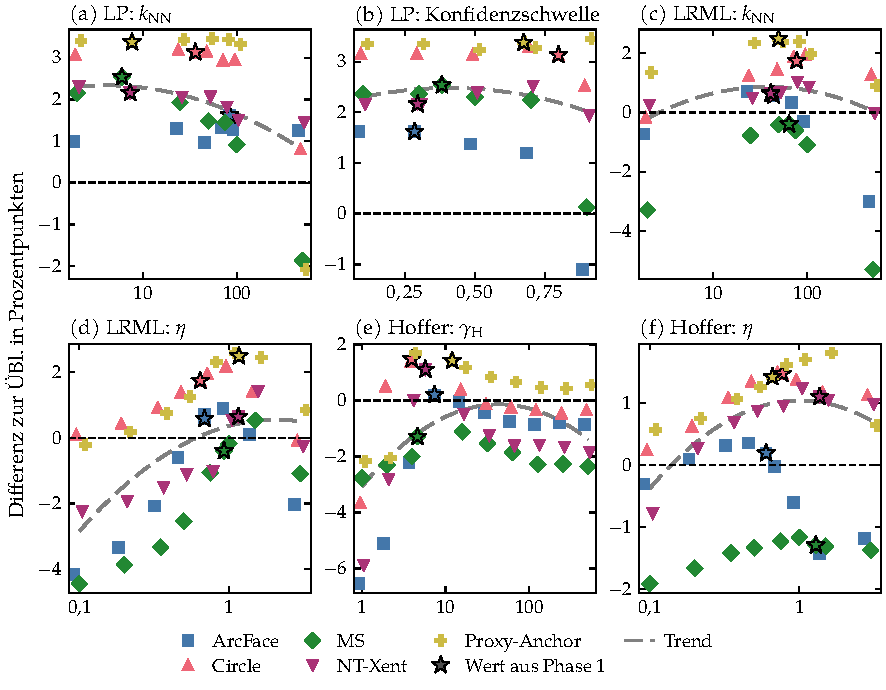
\includegraphics{neu/phase2_sweeps_verluste}
  \caption[Sweeps einzelner Hyperparameter auf Cars196]{Gewinn der Test-\acs{MAP@R} der Einzelmodelle gegenüber der \UEBL bei Variation eines Hyperparameters auf Cars196 ($k=16$, ein Seed, übrige Werte wie in Phase~1). Stern: in Phase~1 gewählter Wert. Grau gestrichelt: Trend über die Verlustfunktionen (quadratische Anpassung an ihren Median je Wert). Logarithmische $x$-Achsen außer bei der Konfidenzschwelle.}
  \label{fig:e:sweeps}
\end{figure}

\begin{figure}[tbp]
  \centering
  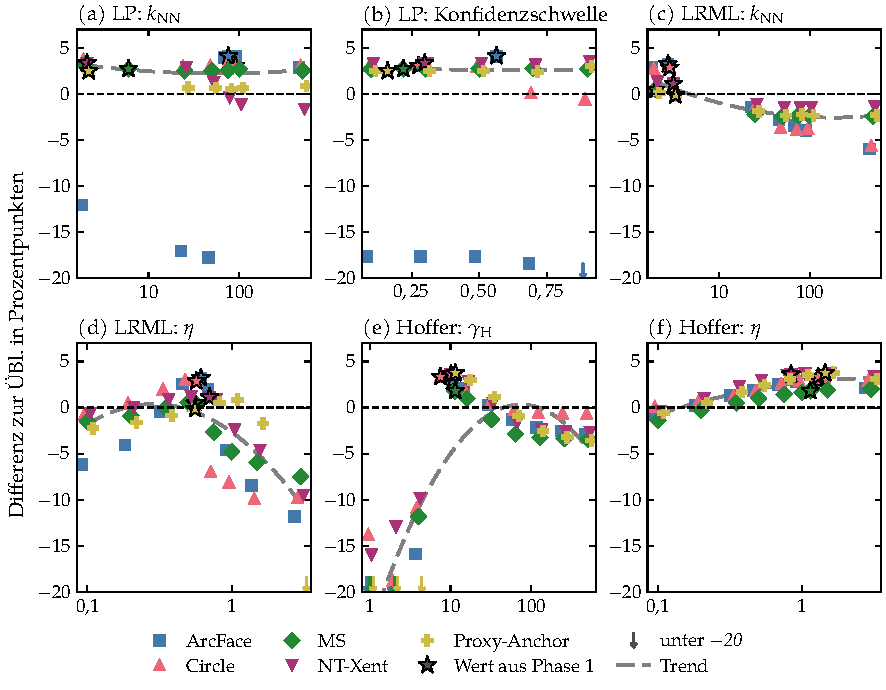
\includegraphics{neu/phase2_sweeps_verluste_inshop}
  \caption[Sweeps einzelner Hyperparameter auf In-Shop]{Sweeps wie in Abbildung~\ref{fig:e:sweeps} auf In-Shop ($k=2$). Die $y$-Achse ist bei \num{-20} Prozentpunkten abgeschnitten, Pfeile markieren Werte darunter. Einzelwerte in Tabelle~\ref{tab:anhang:phase2:inshop}.}
  \label{fig:e:sweeps:inshop}
\end{figure}

Zweitens schadet bei \ac{LRML} ein zu kleines wie ein zu großes $\eta$. Ein kleines $\eta=\num{0.1}$ kostet auf beiden Datensätzen mit jeder Verlustfunktion Leistung, ein großes $\eta=3$ vor allem auf In-Shop, dort um mindestens \num{8.0} Prozentpunkte. Ab welchem Wert die Leistung auf In-Shop einbricht, hängt von der Verlustfunktion ab, mit Circle schon ab $\eta=\num{0.75}$, mit Proxy-Anchor erst bei $\eta=3$.%


Drittens scheitert Hoffer vor allem an einer zu kleinen Distanzskala, wobei eine zu große weniger schadet. Auf In-Shop kosten Distanzskalen $\gamma_{\mathrm{H}}\le4$ mit jeder Verlustfunktion mehr als 13 Prozentpunkte, auf Cars196 Distanzskalen $\gamma_{\mathrm{H}}\le2$ bis zu sieben. Deutliche Verluste treten damit auch oberhalb der notwendigen Mindestskalen aus Abschnitt~\ref{sec:m:hoffer} auf.%


Viertens schadet bei Hoffer auch ein zu kleines $\eta$. Mit $\eta=\num{0.1}$ verliert Hoffer mit jeder Verlustfunktion mehr als die Rauschschwelle, auf In-Shop mindestens \num{3.2} Prozentpunkte. Ein zu großes $\eta$ schadet weniger. Auf In-Shop kostet $\eta=3$ höchstens \num{0.8} Prozentpunkte und auf Cars196 mit ArcFace mehr als einen.%


Wie stark die Mechanismen vom Warm-up abhängen, unterscheidet sich stark. Ohne Warm-up verliert \ac{LRML} mit ArcFace auf beiden Datensätzen und mit \ac{NT-Xent} auf Cars196 sechs bis zehn Prozentpunkte. In den übrigen Kombinationen sind es höchstens \num{2.2}. Hoffer verliert ohne Warm-up höchstens \num{1.0} Prozentpunkte, \ac{SLADE} auf Cars196 höchstens \num{2.1} und auf In-Shop höchstens \num{0.2}.%


Wie robust \ac{LP} gegenüber der Änderung einzelner Hyperparameter ist, hängt von der Verlustfunktion und dem Datensatz ab. Auf Cars196 bleibt \ac{LP} mit Circle, \ac{NT-Xent} und Proxy-Anchor bis 100 Nachbarn, bei allen Konfidenzschwellen und mit jedem Warm-up innerhalb von \num{0.7} Prozentpunkten der regulären Konfiguration. Mit ArcFace und \ac{MS} kosten dagegen hohe Konfidenzschwellen und ein langes Warm-up bis zu \num{2.7} Prozentpunkte, mit \ac{MS} auch 50 und mehr Nachbarn.%


Auf In-Shop ändern die Nachbarzahl, die Konfidenzschwelle und das Warm-up die Leistung von \ac{LP} mit \ac{MS} kaum. Mit Circle schaden nur hohe Konfidenzschwellen, die fast alle ungelabelten Bilder ausschließen. Mit \ac{NT-Xent} und Proxy-Anchor schadet es, mehr als die in Phase~1 gewählten zwei Nachbarn zu verwenden. Mit \ac{MS}, \ac{NT-Xent} und Proxy-Anchor schaden hohe Konfidenzschwellen auch dann nicht, wenn \ac{LP} anfangs nur rund ein bis zwei Drittel der ungelabelten Bilder übernimmt. Dass eine hohe Abdeckung wichtiger ist als die Genauigkeit, gilt damit auf Cars196 für ArcFace und \ac{MS} und auf In-Shop für Circle, mit \ac{MS}, \ac{NT-Xent} und Proxy-Anchor gleichen sich die Abdeckung und die Genauigkeit auf In-Shop aus. Mit ArcFace bricht \ac{LP} auf In-Shop dagegen bei jeder anderen Konfidenzschwelle und bei 2, 25 und 50 Nachbarn ein, um bis zu \num{29.4} Prozentpunkte. Bei 75 und 100 Nachbarn und mit einem anderen Warm-up ändert sich die Leistung kaum. Bei niedrigen Konfidenzschwellen erhält dort jedes ungelabelte Bild sofort ein Pseudo-Label, von denen nur rund ein Drittel richtig ist. Die Validierungsleistung erholt sich davon nicht innerhalb der Patience. Verzögerte Patience (Anhang~\ref{chap:anhang:verzoegerung}) betrifft vier dieser Läufe mit zu früh beendeten Folds. Bei der Schwelle \num{0.5} und bei 25 und 50 Nachbarn ändert sie die Test-\ac{MAP@R} um höchstens \num{0.2} Prozentpunkte, bei der Schwelle \num{0.7} hebt sie sie um \num{7.2} Prozentpunkte, noch immer \num{15.3} unter der regulären Konfiguration. Mit der gewählten Konfidenzschwelle von \num{0.58} übernimmt \ac{LP} dagegen anfangs nur \qty{5}{\percent} der Bilder. Bei den Schwellen \num{0.7} und \num{0.9} sind es nur noch \qty{0.2}{\percent} und auch dort bricht \ac{LP} ein.%


Kein untersuchter Wert verbessert \ac{SLADE} deutlich (Tabelle~\ref{tab:anhang:phase2:slade} in Anhang~\ref{chap:anhang:phase2}). Nur 3 von 215 Läufen liegen über der Rauschschwelle, um höchstens \num{0.5} Prozentpunkte. Auch hier schadet ein großes Zielverhältnis $\eta=3$. Clusterverhältnis und Intervall der Teacher-Aktualisierung ändern die Leistung in 61 von 71 Läufen um weniger als einen Prozentpunkt. Große Einbrüche treten vor allem bei Werten außerhalb der Suchräume der Phase~1 auf, etwa mit Proxy-Anchor auf In-Shop bei einem kleinen Basis-Zielverhältnis, der größte aber innerhalb, bei 512 ungelabelten Bildern je Batch. Beide Einbrüche bleiben auch mit verzögerter Patience die größten (Anhang~\ref{chap:anhang:verzoegerung}).%



Von den vorab festgelegten Erwartungen der Phase~2 (Tabelle~\ref{tab:phase2:eingriffe} und Abschnitt~\ref{sec:m:geometrie}) wurden drei bestätigt, drei nicht bestätigt und sieben teilweise bestätigt. Drei Eingriffe waren ungerichtet (Tabelle~\ref{tab:a:erwartungen}). Bestätigt wurde, dass ein umverdrahteter Graph den Gewinn beseitigt, dass eine zu kleine Distanzskala Hoffer schadet (Abschnitt~\ref{sec:e:sweeps}) und dass \ac{LRML} die Vielfalt der Fold-Modelle erhöht (Abschnitt~\ref{sec:e:phase2:concat}). Nicht bestätigt wurden die Erwartungen, nach denen die Leistung von \ac{LP} umgekehrt U-förmig von der Nachbarzahl abhängt, ein langes Warm-up \ac{LP} nützt und die Referenz bei kleinem Budget stärker komprimiert (Abschnitt~\ref{sec:e:geometrie}).%


\subsection{Einzelmodell und Ensemble in den Ablationen}
\label{sec:e:phase2:concat}

Die bisherigen Befunde der Phase~2 beruhen auf den Einzelmodellen (Mean). Im Ensemble, also mit der Concat-\ac{MAP@R} (Tabellen~\ref{tab:anhang:phase2:concat} und~\ref{tab:anhang:phase2:inshop:concat}), bleiben sie in ihrer Richtung erhalten. Von den 233 Unterschieden, die als Einzelmodell über der Rauschschwelle liegen, liegen 215 auch im Ensemble darüber und keiner kehrt sich um. Deutlich anders fällt das Ensemble wie schon in Phase~1 bei \ac{LRML} aus. Die reguläre Konfiguration gewinnt dort im Ensemble mit mehr Verlustfunktionen und ohne ungelabelte Bilder liegt \ac{LRML} im Ensemble in neun der zehn Kombinationen um mehr als die Rauschschwelle darunter.%


Worauf der größere Ensemble-Gewinn von \ac{LRML} beruht, zeigt die $2\times2$-Zerlegung auf Cars196 beim kleinsten Budget $k=4$, wo der Abstand zwischen Concat und Mean in Phase~1 am weitesten über dem der \UEBL liegt (Tabelle~\ref{tab:e:k4ensemble}). Der Abstand der regulären Konfiguration ist in allen 25 Paaren aus Verlustfunktion und Seed größer als bei der \UEBL. Die eigens gesuchten Hyperparameter der \ac{LRML}-Konfiguration allein erklären das kaum. Mit ihnen und abgeschaltetem \ac{SSL}-Term liegt \ac{LRML} als Einzelmodell in allen 25 Paaren unter der \UEBL. Sein Abstand zwischen Concat und Mean ist dabei kaum größer als bei der \UEBL. Den Abstand vergrößern vielmehr der Term auf den gelabelten Bildern und die ungelabelten Bilder. Die ungelabelten Bilder heben das Ensemble dabei stärker als das Einzelmodell.%


\begin{table}[tbp]
\centering
\caption[Ensemble-Gewinn von \acs{LRML} bei $k=4$]{$2\times2$-Zerlegung von \acs{LRML} auf Cars196 bei $k=4$ mit der Kontrolle mit abgeschaltetem \acs{SSL}-Term: Test-MAP@R (Mean, Concat) in \%, ihr Abstand in Prozentpunkten und der Anteil falscher Nachbarn eines Fold-Modells unter den ersten $R_q$ Treffern, die ein anderes ebenfalls zurückgibt, in \%. Mittel über die fünf Verlustfunktionen und die fünf Seeds. Bezeichnungen wie in den Tabellen~\ref{tab:phase2:eingriffe} und~\ref{tab:m:2x2}.}
\label{tab:e:k4ensemble}
\small
\begin{tabular}{@{}l *{3}{S[table-format=2.1]} S[table-format=2.1]@{}}
\toprule
{Konfiguration} & {Mean} & {Concat} & {Concat $-$ Mean} & {geteilte Fehler} \\
\midrule
\UEBL & 32.6 & 34.9 & 2.3 & 51.9 \\
SSL-Term abgeschaltet & 30.4 & 33.2 & 2.8 & 48.4 \\
ohne ungelabelte Bilder & 30.7 & 34.2 & 3.5 & 43.1 \\
Hyperparameter der \UEBL & 34.7 & 38.2 & 3.4 & 46.8 \\
regulär & 33.4 & 38.3 & 4.9 & 36.9 \\
\bottomrule
\end{tabular}
\end{table}


Der Abstand zwischen Concat und Mean folgt dem Anteil gemeinsamer Fehler. Bei der \UEBL hat ein anderes Fold-Modell im Mittel rund die Hälfte der falschen Nachbarn eines Fold-Modells ebenfalls unter seinen ersten $R_q$ Treffern. Bei der regulären Konfiguration von \ac{LRML} ist es nur gut ein Drittel. Der Anteil ist in allen 25 Paaren kleiner. Auch diesen Anteil senken vor allem der Term und die ungelabelten Bilder. Über alle 125 Läufe hängen der Anteil und der Abstand eng zusammen (Rangkorrelation \num{-0.99}). Die Fold-Modelle von \ac{LRML} irren sich also seltener gleich, sodass sich ihre Fehler im Ensemble eher ausgleichen. Da die Ähnlichkeit im Ensemble das Mittel der Ähnlichkeiten der vier Heads ist, folgt der enge Zusammenhang zum Teil schon aus der Konstruktion von Concat.%





\section{Geometrie des Embedding-Raums}
\label{sec:e:geometrie}
Für Cars196 zeigen Tabelle~\ref{tab:e:geometrie}, Abbildung~\ref{fig:e:geo:budget} und Abschnitt~\ref{sec:e:verlauf} das Mittel über alle fünf Verlustfunktionen und die vier Folds, Anhang~\ref{chap:anhang:geometrie} die Werte je Verlustfunktion, weitere Verläufe und die Streudiagramme zur Korrelationsanalyse. Abschnitt~\ref{sec:e:geo:weitere} zeigt die Geometrie auf Semi-iNat-2021 und den beiden In-Shop-Serien. Die Test-\ac{MAP@R}-Werte dieses Abschnitts stammen aus diesen Läufen mit einem Seed und nicht aus den Mittelwerten über fünf Seeds der vorherigen Abschnitte.

\subsection{Geometrie nach dem Training}
\begin{table}[tbp]
\centering
\caption[Geometrie des Embedding-Raums nach dem Training]{Geometrie des Trainingspools nach dem Training (Cars196, Seed~2, Mittel über die fünf Verlustfunktionen und die vier Folds), Maße wie in Abschnitt~\ref{sec:geometrie}. Head ($-1$): vor dem ersten Optimierungsschritt, Epoche: Mittel der gewählten Epochen, MAP@R: Test-MAP@R (Mean) in \%.}
\label{tab:e:geometrie}
\begin{tabular}{@{}ll S[table-format=1.2] S[table-format=1.2] S[table-format=1.2] S[table-format=1.2] S[table-format=3.0] S[table-format=2.1]@{}}
\toprule
{$k$} & {Modell} & {$\rho$} & {$\pi_{\mathrm{intra}}$} & {$\pi_{\mathrm{inter}}$} & {$\pi_{\mathrm{ratio}}$} & {Epoche} & {MAP@R} \\
\midrule
{--} & DINOv2 & 0.38 & 0.50 & 0.67 & 0.75 & {--} & 20.3 \\
{--} & Head ($-1$) & 0.77 & 0.49 & 0.68 & 0.73 & {--} & 20.1 \\
\addlinespace
4 & \UEBL & 0.78 & 0.48 & 0.86 & 0.56 & 21 & 32.5 \\
 & LP & 1.25 & 0.25 & 0.85 & 0.30 & 115 & 40.1 \\
 & \acs{LRML} & 1.30 & 0.34 & 0.80 & 0.43 & 44 & 32.5 \\
 & Hoffer & 0.86 & 0.48 & 0.99 & 0.48 & 81 & 35.0 \\
 & SLADE & 0.97 & 0.42 & 0.85 & 0.50 & 34 & 34.4 \\
\addlinespace
32 & \UEBL & 0.97 & 0.25 & 0.91 & 0.27 & 108 & 41.4 \\
 & LP & 1.12 & 0.22 & 0.86 & 0.25 & 130 & 42.4 \\
 & \acs{LRML} & 1.38 & 0.20 & 0.89 & 0.22 & 54 & 42.0 \\
 & Hoffer & 1.12 & 0.26 & 1.01 & 0.25 & 65 & 41.3 \\
 & SLADE & 0.99 & 0.22 & 0.90 & 0.25 & 38 & 41.9 \\
\bottomrule
\end{tabular}
\end{table}


Schon die zufällige Projektion des Heads vor dem ersten Optimierungsschritt verdoppelt den spektralen Abfall gegenüber den DINOv2-Merkmalen, lässt $\pi_{\mathrm{ratio}}$ und die Test-\ac{MAP@R} aber fast unverändert (Tabelle~\ref{tab:e:geometrie}). Jedes Training senkt danach $\pi_{\mathrm{ratio}}$ im Mittel deutlich (Abbildung~\ref{fig:e:geo:budget}), mit Proxy-Anchor unter der \UEBL und unter \ac{SLADE} aber nur wenig. Der spektrale Abfall steigt bei den meisten trainierten Heads, im Mittel am stärksten unter \ac{LRML} und \ac{LP}, dort vor allem mit Proxy-Anchor bzw.\ ArcFace. Unter der \UEBL bleibt er bei $k=4$ mit vier der fünf Verlustfunktionen knapp unter dem Ausgangswert, ebenso unter Hoffer mit \ac{NT-Xent} und Proxy-Anchor.%



Die Referenz komprimiert bei kleinem Budget nicht stärker als die \ac{SSL}-Heads, die vorab festgelegte Erwartung trifft also im Mittel nicht zu. Bei $k=4$ wird die \UEBL früh gewählt, im Mittel bei Epoche~21, \ac{LP} erst bei Epoche~115. Der Head der \UEBL hat dort den kleinsten spektralen Abfall und das größte $\pi_{\mathrm{ratio}}$ aller trainierten Heads (Tabelle~\ref{tab:e:geometrie}), nur mit Proxy-Anchor haben Hoffer und \ac{SLADE} einen kleineren spektralen Abfall als die \UEBL. Bei $\pi_{\mathrm{ratio}}$ hängt diese Reihenfolge nicht an einzelnen Verlustfunktionen, denn \ac{LP} hat bei $k=4$ mit jeder den kleinsten Wert und die \UEBL mit vier der fünf den größten. Mit wachsendem $k$ wird die Referenz später gewählt, ihr spektraler Abfall steigt und ihr $\pi_{\mathrm{ratio}}$ sinkt.%


\begin{figure}[tbp]
  \centering
  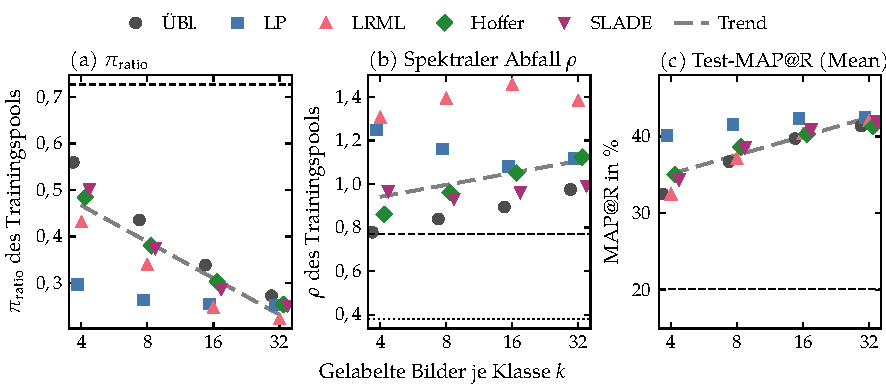
\includegraphics{neu/geometrie_budget}
  \caption[Geometrie des Embedding-Raums über das Label-Budget]{Geometrie des Trainingspools nach dem Training über das Label-Budget (Cars196, Seed~2, Mittel über die fünf Verlustfunktionen und die vier Folds). (a)~$\pi_{\mathrm{ratio}}$, (b)~spektraler Abfall $\rho$, (c)~Test-\acs{MAP@R} der Einzelmodelle. Schwarz gestrichelt: Head vor dem ersten Optimierungsschritt, gepunktet in (b): DINOv2-Merkmale. Grau gestrichelt: Trend über die fünf Verfahren (lineare Anpassung an ihren Median je Budget).}
  \label{fig:e:geo:budget}
\end{figure}

\ac{LP} erreicht schon bei $k=4$ fast dasselbe $\pi_{\mathrm{ratio}}$ wie die Referenz bei $k=32$ und eine Test-\ac{MAP@R} zwischen der Referenz bei $k=16$ und bei $k=32$. Unter den übrigen Verfahren ordnet $\pi_{\mathrm{ratio}}$ die Leistung bei $k=4$ dagegen nicht und auch der spektrale Abfall ordnet die Verfahren nicht nach ihrer Leistung. So erzeugt \ac{LRML} nach \ac{LP} die kompaktesten Klassen, erreicht bei $k=4$ aber nur die Test-\ac{MAP@R} der Referenz.%




\subsection{Verlauf über das Training}
\label{sec:e:verlauf}

Bei $k=4$ rücken unter der Referenz in der ersten Epoche alle Bilder innerhalb ihrer Klassen zusammen, danach entwickeln sich die gelabelten Bilder, die ungelabelten Bilder und die Validierungsklassen unterschiedlich. Bis Epoche~21, der im Mittel gewählten Epoche, werden nur die gelabelten Bilder weiter kompakter, bis auf ein $\pi_{\mathrm{intra}}$ von \num{0.17}, während die ungelabelten Bilder und die Validierungsklassen wieder stärker streuen. Der Head passt sich also an die wenigen gelabelten Bilder an und diese Anpassung überträgt sich nicht auf die übrigen Bilder derselben Klassen und auf ungesehene Klassen.%




Unter \ac{LP} werden dagegen auch die ungelabelten Bilder und die Validierungsklassen kompakter, sobald die Pseudo-Labels einsetzen. Mit ihnen steigen der Anteil ungelabelter Bilder mit richtigem Prototyp und die Validierungs-\ac{MAP@R} deutlich. Wie bei den Budgets der Phase~2 (Abschnitt~\ref{sec:e:nachbarschaft}) wird dabei auch der \ac{kNN}-Graph, aus dem \ac{LP} die Pseudo-Labels berechnet, mit jeder Verlustfunktion reiner. Mit ArcFace und Circle, deren Graphen 92 bzw.\ 38 Nachbarn haben, verlaufen am Ende des Warm-ups nur 39 bzw.\ \qty{58}{\percent} der Kanten innerhalb einer Klasse, die ersten Pseudo-Labels sind aber zu 66 bzw.\ \qty{78}{\percent} richtig. Mit \ac{MS}, \ac{NT-Xent} und Proxy-Anchor, deren Graphen 6 bis 7 Nachbarn haben, liegt die Kantenreinheit etwas über der Genauigkeit der ersten Pseudo-Labels.%


\ac{LRML}, Hoffer und \ac{SLADE} erreichen eine niedrigere Validierungs-\ac{MAP@R}. Mit diesen drei Mechanismen bleiben die ungelabelten Bilder weniger kompakt als mit \ac{LP}, am wenigsten mit Hoffer. Auch liegen weniger ungelabelte Bilder dem Prototyp ihrer Klasse am nächsten als mit \ac{LP}. Unter \ac{LRML} rücken die Klassenmittelpunkte nach dem Warm-up mit vier der fünf Verlustfunktionen zudem wieder zusammen, ebenso unter \ac{SLADE} mit Circle, unter \ac{LP} und Hoffer dagegen nicht. Der Graph von \ac{LRML} wird vor allem während des Warm-ups reiner (Tabelle~\ref{tab:a:reinheit:lrml}). Der spektrale Abfall steigt bei allen Verfahren im Laufe des Trainings, auch dort, wo die Validierungsleistung steigt. Er trennt die Überanpassung der Referenz damit nicht von einem nützlichen Training (Abbildung~\ref{fig:a:rho}). Bei $k=32$ streuen die ungelabelten Bilder unter der \UEBL nicht wieder stärker (Abbildung~\ref{fig:a:verlauf32}).%



\subsection{Semi-iNat-2021 und In-Shop}
\label{sec:e:geo:weitere}

\looseness=-1 Tabelle~\ref{tab:a:geometrie:weitere} in Anhang~\ref{chap:anhang:geometrie} zeigt die Geometrie auf Semi-iNat-2021 und beiden In-Shop-Serien. Auf Semi-iNat-2021 werden bei $k=2$ alle Verfahren außer \ac{LP} früh gewählt und unter der \UEBL, \ac{LRML}, Hoffer und \ac{SLADE} streuen die Klassen des Trainingspools stärker als vor dem Training ($\pi_{\mathrm{intra}}$ \num{0.66} bis \num{0.67} gegenüber \num{0.61}). Nur unter \ac{LP} werden sie kompakter (\num{0.58}) und \ac{LP} erreicht die höchste Test-\ac{MAP@R}. Auf In-Shop trennt dagegen jedes Training die Klassen deutlich. Dabei rücken die Klassenmittelpunkte auseinander. \ac{LP} und Hoffer ordnen dort die meisten ungelabelten Bilder dem richtigen Prototyp zu und erreichen die höchste Test-\ac{MAP@R}. In der Serie mit gelabelten Klassen machen \ac{LP} und \ac{SLADE} die ungelabelten Bilder kompakter als die \UEBL, rücken die Klassenmittelpunkte aber deutlich weniger auseinander. Bei 5 und \qty{10}{\percent} gelabelter Klassen hält \ac{LRML} die Mittelpunkte weiter auseinander und erreicht die höchste Test-\ac{MAP@R}, bei 25 und \qty{50}{\percent} liegen die \UEBL und Hoffer vorn. Auch auf diesen Datensätzen trifft die vorab festgelegte Erwartung nicht zu, beim kleinsten Budget hat der Head der \UEBL nirgends den größten spektralen Abfall.%


\subsection{Zusammenhang mit der Retrieval-Leistung}

\looseness=-1 Tabelle~\ref{tab:e:korrelation} setzt die Geometrie nach dem Training in Beziehung zur Test-\ac{MAP@R}, für jeden Datensatz über alle Kombinationen aus Verfahren, Verlustfunktion und Budget und innerhalb jedes Budgets. Auf Cars196 ist der Zusammenhang mit $\pi_{\mathrm{ratio}}$ des Trainingspools über alle 100 Kombinationen stark und negativ, mit einer Korrelation nach Pearson von \num{-0.86} und nach Spearman von \num{-0.80}. Innerhalb der Budgets wird er mit wachsendem $k$ schwächer und ist bei $k=32$ nur noch schwach (\num{-0.12}), weil dort $\pi_{\mathrm{intra}}$ und $\pi_{\mathrm{inter}}$ beide negativ mit der Test-\ac{MAP@R} zusammenhängen und sich im Verhältnis aufheben.

\begin{table}[tbp]
\centering\small\setlength{\tabcolsep}{4pt}
\caption[Korrelation der Geometrie mit der Retrieval-Leistung]{Rangkorrelation nach Spearman zwischen Maßen nach dem Training und der Test-MAP@R (Mean), Seed 2, Mittel über vier Folds. Gesamt: alle gültigen Kombinationen aus Verfahren, Verlustfunktion und Budget eines Datensatzes, darunter je Budget, Anzahl: Zahl dieser Kombinationen. In der In-Shop-Serie mit gelabelten Klassen steht der Anteil gelabelter Klassen für das Budget. Prototyp: Anteil der ungelabelten Bilder mit richtigem nächstem Klassenprototyp, in dieser Serie nicht definiert (--).}
\label{tab:e:korrelation}
\begin{tabular}{@{}l r S[table-format=-1.2] S[table-format=-1.2] S[table-format=-1.2] S[table-format=-1.2] @{\hspace{12pt}} S[table-format=-1.2] S[table-format=-1.2] S[table-format=-1.2] @{\hspace{12pt}} S[table-format=-1.2]@{}}
\toprule
& & \multicolumn{4}{c}{\textbf{Trainingspool}} & \multicolumn{3}{c}{\textbf{Validierungsklassen}} & {\textbf{Ungelabelt}} \\
\cmidrule(lr){3-6}\cmidrule(lr){7-9}\cmidrule(l){10-10}
& {Anzahl} & {$\pi_{\mathrm{intra}}$} & {$\pi_{\mathrm{inter}}$} & {$\pi_{\mathrm{ratio}}$} & {$\rho$} & {$\pi_{\mathrm{intra}}$} & {$\pi_{\mathrm{inter}}$} & {$\pi_{\mathrm{ratio}}$} & {Prototyp} \\
\midrule
\multicolumn{10}{@{}l}{\textbf{Cars196}} \\*
\quad \textit{gesamt} & 100 & -0.72 & 0.03 & -0.80 & 0.22 & -0.60 & 0.04 & -0.71 & 0.87 \\
\cmidrule{1-10}
\quad $k=4$ & 25 & -0.56 & 0.15 & -0.80 & 0.28 & -0.49 & 0.19 & -0.73 & 0.77 \\
\quad $k=8$ & 25 & -0.51 & 0.07 & -0.68 & 0.32 & -0.40 & 0.04 & -0.61 & 0.72 \\
\quad $k=16$ & 25 & -0.50 & -0.28 & -0.50 & 0.05 & -0.45 & -0.20 & -0.48 & 0.45 \\
\quad $k=32$ & 25 & -0.51 & -0.55 & -0.21 & -0.40 & -0.60 & -0.59 & -0.31 & 0.36 \\
\midrule
\multicolumn{10}{@{}l}{\textbf{Semi-iNat-2021}} \\*
\quad \textit{gesamt} & 100 & -0.80 & 0.14 & -0.80 & 0.74 & -0.69 & 0.12 & -0.51 & 0.95 \\
\cmidrule{1-10}
\quad $k=2$ & 25 & -0.23 & 0.17 & -0.09 & 0.13 & -0.24 & 0.24 & -0.12 & 0.17 \\
\quad $k=4$ & 25 & -0.14 & 0.27 & -0.19 & 0.23 & -0.09 & 0.24 & -0.13 & 0.35 \\
\quad $k=16$ & 25 & 0.24 & 0.10 & 0.41 & -0.63 & 0.20 & 0.03 & 0.46 & 0.69 \\
\quad $k=100$ & 25 & 0.42 & 0.25 & 0.33 & -0.45 & 0.46 & 0.21 & 0.37 & 0.84 \\
\midrule
\multicolumn{10}{@{}l}{\textbf{In-Shop}} \\*
\quad \textit{gesamt} & 50 & -0.10 & -0.03 & -0.37 & 0.21 & -0.04 & -0.05 & -0.31 & 0.89 \\
\cmidrule{1-10}
\quad $k=2$ & 25 & -0.11 & -0.12 & -0.32 & 0.55 & -0.04 & -0.18 & -0.23 & 0.94 \\
\quad $k=4$ & 25 & 0.38 & -0.17 & 0.45 & -0.17 & 0.37 & -0.17 & 0.45 & 0.67 \\
\midrule
\multicolumn{10}{@{}l}{\textbf{In-Shop mit gelabelten Klassen}} \\*
\quad \textit{gesamt} & 97 & -0.24 & 0.31 & -0.62 & 0.45 & -0.15 & 0.31 & -0.53 & {--} \\
\cmidrule{1-10}
\quad \qty{5}{\percent} & 25 & 0.06 & 0.13 & -0.12 & -0.02 & 0.08 & 0.13 & -0.10 & {--} \\
\quad \qty{10}{\percent} & 25 & 0.17 & 0.31 & -0.22 & 0.09 & 0.19 & 0.32 & -0.20 & {--} \\
\quad \qty{25}{\percent} & 24 & 0.66 & 0.63 & 0.13 & 0.05 & 0.69 & 0.61 & 0.17 & {--} \\
\quad \qty{50}{\percent} & 23 & 0.59 & 0.60 & 0.17 & -0.06 & 0.65 & 0.59 & 0.29 & {--} \\
\bottomrule
\end{tabular}
\end{table}


Mit dem spektralen Abfall besteht auf Cars196 kein linearer Zusammenhang. Am engsten hängt auf allen Datensätzen über alle Kombinationen die Genauigkeit der Prototypen-Zuordnung auf den ungelabelten Bildern mit der Test-\ac{MAP@R} zusammen (Tabelle~\ref{tab:e:korrelation}). Für diese Größe war vorab keine Erwartung festgelegt. Auf Semi-iNat-2021 und In-Shop hängt $\pi_{\mathrm{ratio}}$ über alle Budgets ebenfalls negativ mit der Test-\ac{MAP@R} zusammen, innerhalb der Budgets aber nur bei kleinem $k$. Auf Semi-iNat-2021 ist der Zusammenhang bei $k=2$ und 4 negativ (\num{-0.49} und \num{-0.41}), bei $k=16$ und 100 schwach positiv, auf In-Shop bei $k=2$ negativ und bei $k=4$ positiv. In der In-Shop-Serie mit gelabelten Klassen liegt er innerhalb der Anteile zwischen \num{-0.15} und \num{0.13}. Abschnitt~\ref{sec:d:ablationen} ordnet diese Zusammenhänge ein. Die Prototypen-Genauigkeit hängt dagegen in jedem Budget positiv mit der Test-\ac{MAP@R} zusammen, auf Semi-iNat-2021 mit \num{0.81} bis \num{0.89}. Auf Cars196 hängt bei kleinen Budgets zudem die Dauer des Trainings mit der Test-\ac{MAP@R} zusammen, mit einer Rangkorrelation zwischen gewählter Epoche und Test-\ac{MAP@R} von \num{0.61} bei $k=4$, bei $k=32$ nicht mehr.%




\section{Sensitivität der Hyperparameter, Rechenzeit und Speicherbedarf}
\label{sec:e:sensitivitaet}
\label{sec:e:aufwand}

Die Optima der Phase-1-Suchen sind flach. Im Median liegen 12 bis 48 der 80 Versuche einer Suche höchstens einen Prozentpunkt hinter dem besten und der zweitbeste Versuch nur \num{0.02} bis \num{0.13} Prozentpunkte dahinter. Innerhalb eines Standardfehlers der Fold-Werte des besten Versuchs liegen im Median auf \ac{CUB} 79 der 80 Versuche, auf Cars196 44, auf Semi-iNat-2021 25, auf In-Shop 6 und in der In-Shop-Serie mit gelabelten Klassen 4. Die exakten Werte einer gewählten Konfiguration sind deshalb nicht interpretierbar, nur der Bereich guter Werte. Auf den zufälligen Versuchen heben sich nur wenige Hyperparameter vom Rauschen ab, vor allem die Skalen von Proxy-Anchor, ArcFace und Circle, die Temperatur von \ac{NT-Xent} mit wechselndem Vorzeichen, die Distanzskala von Hoffer sowie das Warm-up und das Zielverhältnis $\eta$ von \ac{LRML} und $\eta$ von \ac{SLADE}. Die vier Parameter des Graphen und der Pseudo-Labels bei \ac{LP} heben sich nur in 10 ihrer 100 Kombinationen aus Parameter und Suche ab. Das schließt lokale Abhängigkeiten oder Wechselwirkungen nicht aus, wie die Einbrüche mit ArcFace auf In-Shop in den Sweeps zeigen.%


Die Mechanismen verlängern einen Trainingsschritt unterschiedlich stark, Hoffer am meisten. Auf In-Shop bei $k=2$ (Abschnitt~\ref{sec:m:aufwand}) dauert ein Schritt nach dem Warm-up mit der \UEBL \num{3.3} Millisekunden, mit \ac{LP} und \ac{LRML} \num{4.7} bzw.\ \num{6.3}, mit \ac{SLADE} \num{16.2} und mit Hoffer \num{24.8} Millisekunden. Eine Epoche einschließlich der Neuberechnung des Graphen, der Pseudo-Labels oder der Cluster und der Validierung dauert mit der \UEBL \num{0.6} Sekunden, mit \ac{LRML} \num{1.6}, mit \ac{LP} und \ac{SLADE} \num{2.6} bzw.\ \num{2.7} und mit Hoffer \num{3.9} Sekunden. Die Folds der Phase~1 trainieren dort im Median 155 bis 258 Epochen, am längsten mit der \UEBL und \ac{LP}. Mit diesen Epochen und den gemessenen Raten dauert ein Fold im Median \num{2.0}~Minuten mit der \UEBL, \num{3.4} mit \ac{LRML}, \num{6.8} mit \ac{SLADE}, \num{8.9} mit \ac{LP} und \num{10.4} mit Hoffer.%

Beim Speicherbedarf fällt nur \ac{NT-Xent} auf (Abschnitt~\ref{sec:m:verluste}). Ein Trainingsschritt belegt im Spitzenwert bei Batchgröße 256 und \ac{SPC}-4 rund \SI{0.7}{\giga\byte} zusätzlich, bei 512 und \ac{SPC}-2 rund \SI{1.8}{\giga\byte} und bei 512 und \ac{SPC}-8 rund \SI{12}{\giga\byte} (Abschnitt~\ref{sec:m:aufwand}). Die übrigen vier Verlustfunktionen bleiben bei dieser größten Kombination bei rund \SI{0.1}{\giga\byte} oder weniger.%

